\documentclass[a4paper,12pt]{article}

\usepackage[utf8]{inputenc}
\usepackage{polski}
\usepackage[T1]{fontenc}

\usepackage{graphicx} 
\usepackage[export]{adjustbox}
\usepackage{wrapfig} 
\usepackage{subcaption}
\usepackage{amssymb}
\usepackage{setspace}
\usepackage{datetime}
\usepackage{mathptmx}
\usepackage{tocloft}
\usepackage{blindtext}

\usepackage{hyperref}


\urlstyle{colorlinks=true,
    linkcolor=blue,
    filecolor=magenta,      
    urlcolor=cyan,
    pdftitle={Sharelatex Example},
    bookmarks=true,
    pdfpagemode=FullScreen,}

\newcommand{\MONTH}{%
  \ifcase\the\month
  \or Styczeń % 1
  \or Luty % 2
  \or Marzec % 3
  \or Kwiecień % 4
  \or Maj % 5
  \or Czerwiec % 6
  \or Lipiec % 7
  \or Sierpień % 8
  \or Wrzesień % 9
  \or Październik % 10
  \or Listopad % 11
  \or Grudzień % 12
  \fi}
\makeatletter
\newcommand{\YEAR}{\@Roman{\the\year}}
\makeatother

\usepackage[left=2.5cm, right=2.5cm, top=2.5cm, bottom=2cm]{geometry}
\setlength{\parindent}{4em}
\setlength{\parskip}{1pt}
\renewcommand{\baselinestretch}{1.5}
\renewcommand{\cftsecleader}{\cftdotfill{\cftdotsep}}
%?
\usepackage[11pt]{moresize}
\prefixing

\author{Przemysław Woldon}
\date{}

\begin{document}
    %strona tytułowa
    \begingroup
        \fontsize{12pt}{0.2}\selectfont
            \begin{center}Politechnika Łódzka\end{center}
            \begin{center}Wydział Elektrotechniki, Elektroniki, Informatyki i Automatyki\end{center} 
            \begin{center}Instytut Informatyki Stosowanej\end{center} 
        
        \vspace*{125px}     
    
        \fontsize{14pt}{0.2}\selectfont
            \begin{center}\textbf{PRACA DYPLOMOWA INŻYNIERSKA}\end{center} 

        \vspace*{50px}

        \fontsize{12pt}{0.2}\selectfont
            \begin{center}System umożliwiający digitalizację zapisów nutowych pieśni, \\\vspace{3mm} ułatwiający ich przechowywanie i przetwarzani\end{center} \vspace{5mm}
            \begin{center}A system for digitization of sheet music facilitating their storage and processing\end{center} 

        \vspace*{50px}

        \fontsize{12pt}{0.2}\selectfont 
            \begin{center}Przemysław Woldon\end{center} 
            \begin{center}Numer albumu: 195092\end{center} 

        \vspace*{70px}
        
        \fontsize{12pt}{0.2}\selectfont 
            \begin{flushright}Opiekun pracy:\end{flushright} 
            \begin{flushright}Dr. inż. Paweł Kapusta\end{flushright} 
    
        \vspace*{90px}

        \fontsize{12pt}{0.2}\selectfont 
            \begin{center}Łódź, \MONTH \vspace{2cm}  \the\year \end{center} 
    \endgroup
    \pagenumbering{gobble}
    \newpage
    \pagenumbering{arabic}
	\setcounter{page}{2}
    \tableofcontents
	\newpage 

    %\setcounter{secnumdepth}{0}
	\section*{Streszczenie}
	\addcontentsline{toc}{section}{Streszczenie}
	\section*{Abstract}
    \addcontentsline{toc}{section}{Abstract}    
    %\setcounter{secnumdepth}{1}
    
	\newpage 

	\section{Wstęp}
			\paragraph{\indent} Obecnie coraz częściej w świątyniach możemy spotkać się z rzutnikami lub wyświetlaczami led, na których ekranizowane są teksty pieśni.
				Cyfrowe zbiory pieśni dostarczane przez producentów wyświetlaczy nie są w stanie sprostać wymaganią jakie stawia przed nimi: dynamiczny rozwój muzyki - powstawaniu nowych utworów, zróżnicowanym tradycjom lokalnym oraz indywidualnym upodobaniom muzyków kościelnych wykorzystującym różne śpiewniki.
				Czasochłonny proces budowy wspomnianych zbiorów często
				polega na ręcznym przepisywaniu tekstów pieśni z wykorzystywanych przez muzyków kościelnych śpiewników.
				Automatyzacja tego procesu pozwoli na łatwiejsze dopasowanie zbiorów do potrzeb muzyków kościelnych i tradycji lokalnych. 
				\par Dzięki pracy nad tą aplikacją autor mógł połączyć swoje dwie pasje --- muzykę kościelną i informatykę. Pomysł budowy aplikacji narodził się z zaobserwowania, że osoby odpowiedzialne za muzykę kościelna przeznaczają znaczącą liczbę godzin na ręczne przepisywanie śpiewników, poprawę błędów w już dostarczonych zbiorach. Zaangażowanie technik informatycznych do tego zadania pozwoli nie tylko na zaoszczędzenie czasu, ale również wyeliminuje możliwość wystąpienia błędów spowodowanych przez człowieka.
				Budowa prototypu zapewniającego pełną funkcjonalność, który może być dalej rozwijany daje możliwość jego opublikowania i dotarcia do szerokiego grona interesariuszy.  
		\subsection{Cel pracy}
			\paragraph{\indent}
			 Celem niniejszej pracy dyplomowej było skonstruowanie algorytmów 
				przetwarzających strony śpiewników kościelnych tak aby jak najlepiej przygotować je do optycznego rozpoznania zawartego w nich tekstu. 
				W algorytmach wykorzystane zostały metody przetwarzania obrazów, które redukują szumy, usuwają obszary, które nie zawierają znaczących w analizie danych (eliminacja nadmiarowych informacji), prostują strony, wykrywają i usuwają znaki muzyczne, wykrywają znaki (cyfry, litery, znaki interpunkcyjne), zaś algorytmy cyfrowego rozpoznawania tekstu odczytują wykryte litery uwzględniając polskie znaki diakrytyczne. Dzieki zastosowaniu konwolucyjnych sieci neuronowych wypracowane rozwiąznie zostało uogólnione, a finalne algorytmy umożliwiają pracę na różnych danych wejściowych. Zaś budowa aplikacji uwzględniająca dobre praktyki programowania ułatwi jej dalszy rozwój. 
	\newpage 

	\section{Wykorzystane technologie}
	    \paragraph{\indent} Cyfrowe przetwarzanie obrazów \textit{(ang. digital image processing)} jest dosyć młodą dziedziną nauki zajmującą się reprezentacją obrazu w pamięci komutera, jego akwizycją i przetwarzaniem. 
        \par Obecnie można znaleźć wiele bibliotek umożliwiających pracę z obrazami, na przykład: Imagemagick, Generic Image Library, SIMD i inne. Najbardziej powszechną biblioteką jest bilbioteka OpenCv, dostarcza ona bardzo bogatą, bezkonkurencyjną funkcjonalność, przejrzystą i zawierającą podstawy matematyczne dokumentację, zaś dynamicznie rozwijająca się społeczność zgromadzona wokół biblioteki ułatwia z nią pracę szczególnie nowym użytkownikom.
	    
		\subsection{Biblioteka OpenCv}
			%\paragraph{\indent} 
			%	OpenCv jest biblioteką służącą do komputerowego przetwarzania obrazów oraz uczenia maszynowego, o otwartym kodzie źródłowym.
		\subsubsection{Zarys historyczny}
			\paragraph{\indent}  Prace nad budową tej biblioteki rozpoczął jeden z        pracowników firmy Intel - Gary Rost Bradski, zainspirowany środowiskiem     akademickim, które wówczas posiadało bardzo bogatą                          infrastrukturę służącą do przetwarzania obrazów, jednak                     przeznaczoną dla użytku wewnętrznego. Studenci w obrębie jednej             jednostki akademickiej dzielili się kodem zawierającym gotowe               implementacje algorytmów, co znacząco ułatwiało prace przy własnych         projektach czy aplikacjach. 
				Stąd głównym celem biblioteki OpenCv jest udostępnienie wszystkim zainteresowanym zagadnieniami przetwarzania obrazów i sztucznej inteligencji gotowej jednolitej, darmowej infrastruktury pozwalającej na pracę, tak aby nie trzeba było ponownie ''wynajdywać koła''.\par
				OpenCv zostało przedstawione po raz pierwszy w 1999 roku szerszemu gronu odbiorców. \par  
                 W wersji 1.0 kod biblioteki stanowiły wyłącznie najbardziej użyteczne przy przetwarzaniu obrazów
				algorytmy zaimplementowane w języku C. 
				Od tego czasu biblioteka znacząco się zmieniła. \par
			    W wersji 2.0 znaczący wpływ na wydanie wywarły trendy obecne w prowadzeniu projektów, w których wytwarza się oprogramowanie - repozytorium kodu w systemie kontroli wersji Git, gdzie możemy znaleźć najnowszą wersję biblioteki i najświeższe poprawki, testy jednostkowe czy booty ciągłej kompilacji. 
				Zaimplementowano również interfejsy dla języków programowania takich jak C++ oraz Javy, Python’a, MATLAB-a.
				Od tego czasu nowe typy danych i funkcje metody implementowano w C++, a już napisane w języku C dopasowano do nowej technologii. \par
				Nieustannie zwiększająca się liczba zaimplementowanych algorytmów użytecznych przy przetwarzaniu obrazów przyczyniła się do modułowej budowy biblioteki w wersji 3.0, która przedstawia się w sposób następujący:
                
                \begin{spacing}{1}
    				\begin{itemize}
    					\item (warstwa wierzchnia) system operacyjny,
    					\item interfejsy dla różnych języków i aplikacje,
    					\item moduł \textit {opencv\_contrib} zawierający kod napisany i dołączony do biblioteki przez użytkowników,
    					\item rdzeń OpenCv,
    					\item optymalizacje sprzętowe (warstwa HAL \textit {ang. hardware acceleration layer}).
    				\end{itemize} 
                \end{spacing}
            
				\begin{figure}[!ht]  
					\begin{center}
						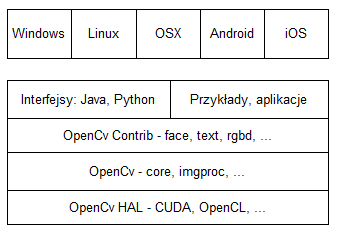
\includegraphics[width=12cm] {image//openCvBudowa.png} 
					\end{center}
					\caption
					    [Budowa modułowa OpenCv]
					    {Budowa modułowa OpenCv}
				\end{figure}

				\par OpenCv w tej wersji wspiera budowanie i dołączanie do biblioteki walsnych modulów.
	            
				\begin{figure}[!ht]   
					\begin{center}
		    				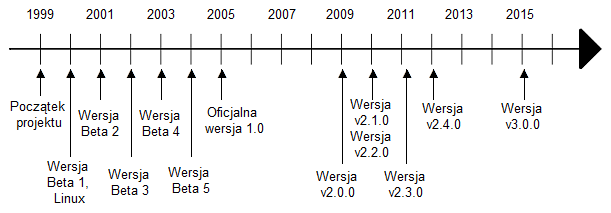
\includegraphics[width=\linewidth] {image//osCzasu.png} 
					\end{center}
					\caption
					    [Rozwój projektu w czasie]  
					    {Rozwój projektu w czasie}  
				\end{figure}


		\subsubsection{Popularność projektu}  
			\paragraph{\indent}
				Projekt cieszy się bardzo dużym powodzeniem, które nieustannie rośnie. Świadczy o tym liczba pobrań 
				wynosząca około 14 milionów razy, zaś miesięcznie około 200 tysięcy.
				Obecnie biblioteka zawiera ponad 2500 zoptymalizowanych algorytmów, które służą do przetwarzania obrazów
				również w czasie rzeczywistym i uczenia maszynowego, co znacząco ułatwia tworzenie aplikacji użytkownikom. 
				Programiści piszący kod uwzględniali wymóg przenośności OpenCv, a więc możliwości kompilacji na każdym odpowiednim kompilatorze języka C++, co wymusiło restrykcyjną zgodność ze standardem i ułatwiło obsługę różnych platform.
				Biblioteka dostępna jest na systemach operacyjnych takich jak: Windows, Linux, Mac OS X, do których dołączyły systemy operacyjne platforma mobilnych (Android i iOS), co znacząco przyczyniło się do zwiększenia liczby użytkowników

		\subsubsection{Zastosowania biblioteki OpenCv}
			\paragraph{\indent} 
			    Dynamiczny rozwój technologiczny otwiera przed biblioteką nowy horyzont użyteczności. OpenCv znajduje zastosowanie w wielu obszarach życia do tego stopnia że wykorzystanie projektu wydaje się rzeczą całkowicie naturalna a wręcz niezauważalną. Biblioteka wykorzystywana jest w:
			
			    \begin{spacing}{1}
			        \begin{itemize}
        				\item skanowaniu kodów QR,
        				\item monitoringu,
        				\item rozpoznawaniu dzwięków i muzyki,
        				\item obrazowaniu medycznym,
        				\item robotyce,	
        				\item przemyśle - produkcji masowej i kontroli jakości,
        				\item wojsku - bezzałogowe pojazdy, fotografie lotnicze,
				        \item analizie obiektów,
				        \item Google Street View,
		            \end{itemize}
                \end{spacing}
    
    	\subsubsection{Reprezentacja obrazów}
	    \paragraph{\indent} Obrazy można podzielić w najprostszy sposób na obrazy barwne i obrazy w skali szarości. Obrazy w bibliotece OpenCv reprezentowane są w postaci macierzy (Mat). Narzędzie to udostępnia bogatą gamę możliwości reprezentacji poszczególnego piksela, a więc i samego obrazu. Tak więc jeden piksel jest reprezentowany w następujący sposób --- CV\_xCy
	    \begin{spacing}{1}
	    \begin{itemize}
	        \item{x --- parametr określający typ}
	            \begin{itemize}
	            \item{8U --- 8---bitowy char bez znaku}
	            \item{16S --- 16---bitowy short ze znakiem}
	            \item{16U --- 16---bitowy short bez znakiu}
	            \item{32S --- 32---bitowa liczba całkowita ze znakiem}
	            \item{32F --- 32---bitowa liczba zmiennoprzecinkowa}
	            \item{64F --- 64---bitowa liczba zmiennoprzecinkowa}
	            \end{itemize}
	        \item{y  --- parametr określający liczbę kanałów}
	            \begin{itemize}
	            \item{1 --- jeden kanał}
	            \item{2 --- dwa kanały}
	            \item{3 --- trzy kanały}
	            \end{itemize}
	    \end{itemize}
	    \end{spacing}
	    lub jeśli użytkownik potrzebuje więcej kanałów może użyć funkcji CV\_xC(n), gdzie n --- liczba kanałów. Można również wybierać z obfitej przestrzeni reprezentacji obrazu np. RGB, RGBA, HSV i innych. \par
	    Obrazy przechowywane jako pliki w pamięci komputera mają różne rozszerzenia, które wpływają na ich jakość, wielkość zajmowanego miejsca na dysku. Przykładowe formaty obrazów: 
        
        \begin{spacing}{1}
            \begin{itemize}
	            \item TIFF (\textit{ang. Tagged-lmage File Format}) --- format standardowy i najbardziej podstawowy, używa algorytmu kompresji bezstratnej;
	            \item 	JPEG (\textit{ang. Joint Photographic Experts Group}) --- używa algorytmu kompresji stratnej;
	            \item PNG (\textit{ang. Portable Network Graphics}) --- używa algorytmu kompresji bezstratnej; 
                \item  GIF (\textit{ang. Graphics Interchange Format}) --- używa algorytmu kompresji bezstratnej LZW (\textit{Lemple-Zif-Welch}), pliki małych rozmiarów, często wykorzystywany do tworzenia animacji;
	        \end{itemize}
	    \end{spacing}
    
    
    \subsection{Konwolucyjne sieci neuronowe}
        \paragraph{\indent} Działanie sztucznych sieci neuronowych                        (\textit{Artificial neural network (ANN)}) opiera się na modelu pojedynczego     neuronu( perceptronu), które zostają łączone w większe struktury.
            Matematyczną podstawę dla działania konwolucyjnych sieci neuronowych (\textit{Convolutional neural networks (CNN)}) stanowi splot (konwolucja) - 
            jest to operacja określana na dwóch funkcjach (np. f(t), g(t)) w wyniku której otrzymujemy nową funkcję (np. h(t)); 
            w przetwarzaniu obrazów jedną z funkcji jest analizowany obraz wejściowy,
            zaś druga filtr.
            Obraz wejściowy przechodzi przez wiele filtrów i każdy z nich mapuje cały obraz wejściowy biorac pod uwage jego części o rozmiarze filtra. Tak wiec konwolucyjne sieci neuronowe uczą się obrazu, analizując go pewnymi wycinkami. Dokładnie filtr przechodzący przez obraz mnoży odpowiednie wartości a następnie sumuje ich iloczyny.
        
            \begin{displaymath}
                h[m, n] = ( f \star g)[m, n] = \sum\limits_{j}\sum\limits_{k}f[j, k]g[m-j, n-k]
            \end{displaymath}
		    
		    \newpage
		    
    	    \begin{figure}[h!]
                \centering
                \begin{subfigure}[b]{0.45\linewidth}
                    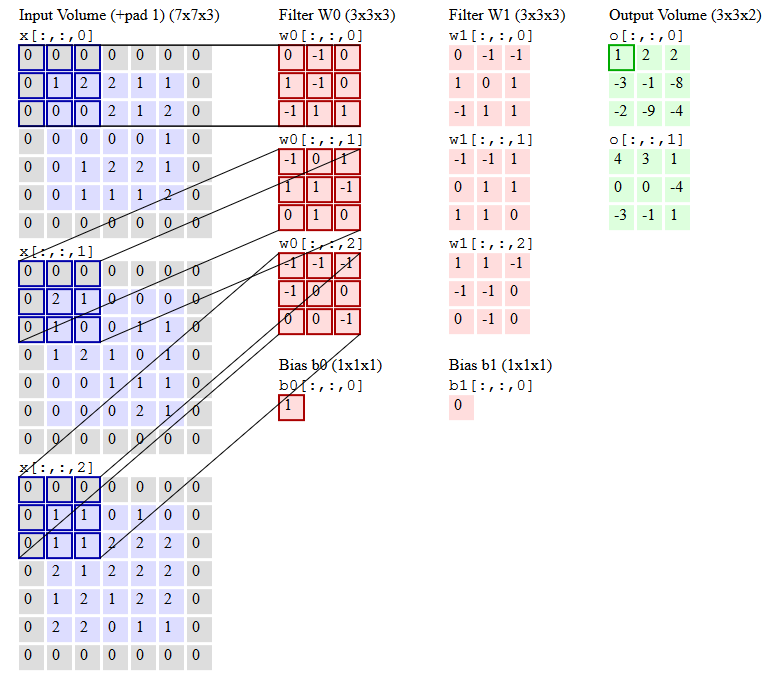
\includegraphics[width=\linewidth]{image//con_01.png}
                \caption{}
                \end{subfigure}
                \begin{subfigure}[b]{0.45\linewidth}
                    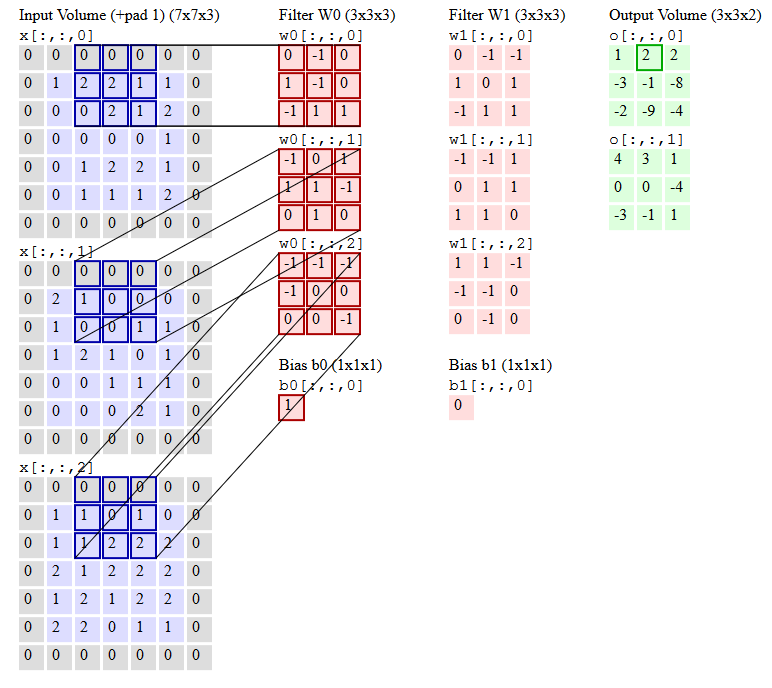
\includegraphics[width=\linewidth]{image//con_02.png}
                \caption{}
                \end{subfigure}
                \newline
                \begin{subfigure}[b]{0.45\linewidth}
                    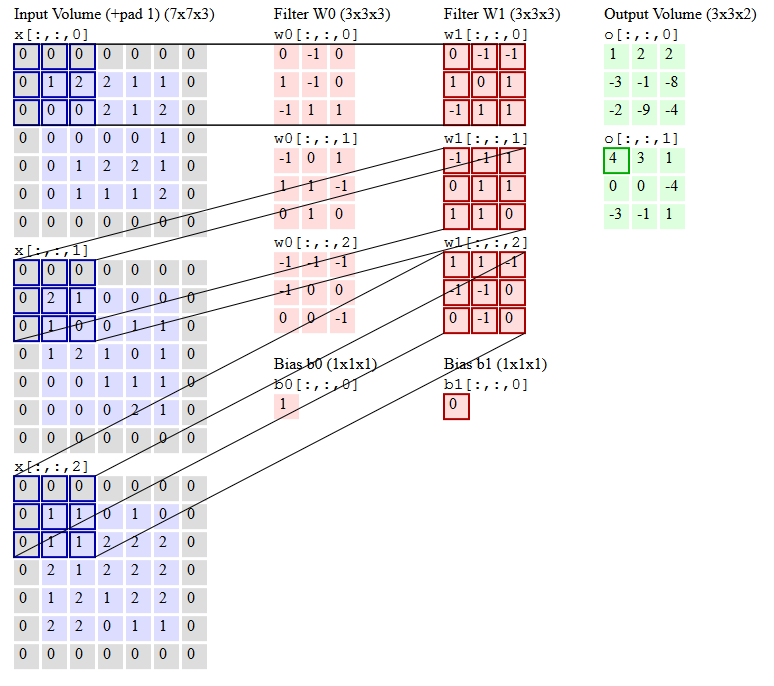
\includegraphics[width=\linewidth]{image//con_03.png}
                \caption{}
                \end{subfigure}
                \begin{subfigure}[b]{0.45\linewidth}
                    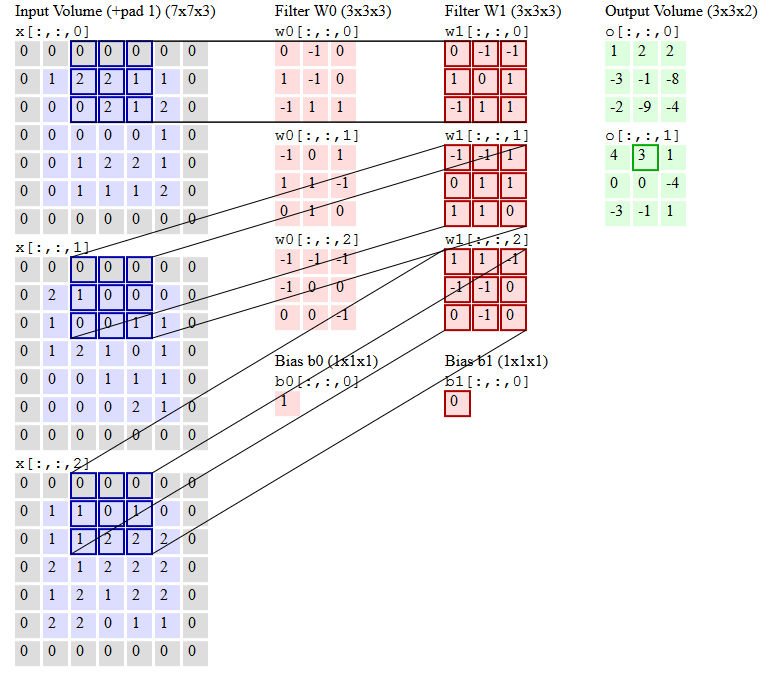
\includegraphics[width=\linewidth]{image//con_04.png}
                \caption{}
                \end{subfigure}
              
                \caption
                    [Przykład działania konwolucji]
                        {Przykład działania konwolucji \\  Źródło: \href{https://skymind.ai//wiki//convolutional-network}{\url{https://skymind.ai//wiki//convolutional-network}}, data dostępu: 09.07.2018}
            \end{figure}
        
        Następnie dane wejściowe przechodzą przez nieliniową transformację (funkcję aktywacji), która określa czy perceptron będzie aktywowany czy nie. Funkcja ta odgrywa znacząca rolę w dopasowaniu gradientów. Funkcje te są ciągłe i różniczkowalne (wyjątek stanowi funkcja ReLU w zerze).
        
        Wśród funkcji aktywacji wyróżniamy funkcje takie jak: funkcja sigmoidalna,  tangens hiperboliczny (\textit{tanh}), rektyfikowana jednostka liniowa (\textit{ang. The Rectified Linear Unit (ReLU)}), 
        które mapują wartość wejsciową w zakresach odpowiednio (0, 1), (-1, 1) i (0, x). Funkcja softmax przetwarza wektor wejściowy na wektor wyjściowy według nastepującego wzoru będącego rozkładem prawdopodobieństwa, mówiącego o prawdopodobieństwie wystąpienia poszczególnej klasy. 
        
        \begin{displaymath}
            \sigma (z)_{j} = \frac{e^{z_{j}}}{ \sum_{k=1}^K e^{z_{j}}}
        \end{displaymath}

        Suma wartości wektora wyjściowego wynosi jeden. Wektor wejsciowy oraz wyjściowy mają taki sam rozmiar. Funkcja normalizuje K wymiarowy wektor w K wymiarowy wektor  $ \sigma (z)$. 
        
	    \par Zjawiskiem występującym przy zastosowaniu konwolucyjnych sieci neuronowych konwolucyjnych jest pooling.
	    Polega on na zmniejszeniu wymiarowości przetwarzanego obrazu. Zaletą zastosowania poolingu jest wyeksponowanie znaczących informacji, które zawiera obraz. Można wyróżnić average pooling i max pooling, mogą one wykonane na każdym z kanałów obrazu z różnym rozmiarem jądra oraz różnym krokiem. 
	 
	    \begin{figure}[!ht]
            \centering
                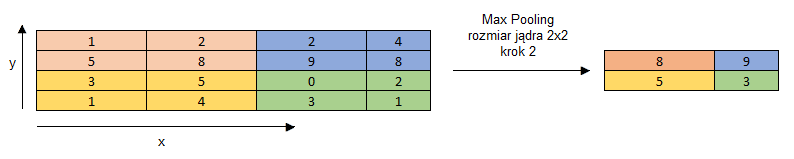
\includegraphics[width=17cm, height=4.5cm]{image//maxPoolingImg.png}
                \caption
                [Max pooling]
                {Max pooling}
        \end{figure}
        
        Pooling jest również metodą regularyzacji sieci neuronowej, zapobiegający jej przeuczeniu. 
        
        \par 
        Inną efektywną drogą regularyzacji sieci neuronowych również zapobiegającą zjawisku przeuczenia się sieci jest dropout. 
        Podczas treningu sieci zostają wykluczone, dezaktywowane nadmiarowe neurony z architektury sieci w sposób losowy, w efekcie może on uwzględniać np. neurony o najmniejszych wagach, które nie mają wiekszego wpływu na ostateczny wynik działania sieci. Tak odrzucone neurony nie biorą już udziału w końcowym procesie wnioskowania. Obok dropout'u istnieją takie metody zapobiegające przeuczeniu się sieci jak: legularyzacja l1 i l2, zmanejszające wartość absolutną, pierwiastek kwadratowy wag, uznając ze modele mające zminimalizowane wagi osiągają lepsze wyniki. Legularyzacja, a w szczególności dropout pozytywnie wpływa na minimalizację błędu klasyfikacji sieci neuronowej. 
        
	    Kolejnym algorytmem powszechnie stosowanym w celu optymalizacji sieci neuronowych (wielowarstwowych) jest algorytm wstecznej propagacji błędów \textit{(ang. backpropagation)}. Wagi poszczególnych połączeń mogą zostać wytrenowane, a więc dobrane automatycznie i stanowiące w przybliżeniu zestaw najbardziej optymalny. Wsteczna propagacja błędów polega na aktualizowaniu wartości wag na podstawie wartości błędu wag dotychczasowych. W celu poprawy efektywności wstecznej propagacji błędów często zaleca się następujące metody: 
        zastosowanie losowych wag początkowych, kilkukrotne powtarzanie procesu uczenia. Sam algorytm uwzględnia następujące kroki zakładając losową generację wag początkowych: obliczenie odpowiedź sieci dla każdego z wektorów uczących, każdy z neuronów wyjściowy oblicza swój błąd, propagacja błędów do warstw wcześniejszych, na podstawie propagowanej wartości błędu każdy z neuronów modyfikuje wagi, powyższe kroki są powtarzane dopóki średni błąd nie przestanie maleć.

        \par Do budowy konwolucyjnych sieci neuronowych został wykorzystany framework Deeplearning4j. Działa na wirtualnej maszynie Javy. Można go wykorzystywać z językiem programowania Java (DL4J) i Scala (DL4S). Narzędzie posiada bogatą dokumentacje, repozytorium kodu na platformie GitHub gdzie znajdują się zaimplementowane gotowe przykłady użycia frameworku \href{https://github.com//deeplearning4j//nd4j}{\url{https://github.com//deeplearning4j//nd4j}}. Umożliwia konfigurację środowiska za pośrednictwem narzędzi automatyzujących budowę projektu, na przykład: Maven, Gradle, Ivy, SBT. Do operacji backendowych narzędzie udostępnia wybór pomiędzy GPU, a CPU. Framework 
        posiada zaimplementowane mechanizmy budowy, regularyzacji, optymalizacji sieci neuronowych, różnorodne rodzaje warstw z których możemy budować architekturę sieci (główne grupy) : Feed-Forward Layers, Output Layers, Convolutional Layers, Recurrent Layers,  Unsupervised Layers, Other Layers, Graph Vertices, InputPreProcessors. W pracy wykorzystywane są następujące z udostępnionych warstw wraz z konfiguracją: 
        \begin{spacing}{1.5}
        \begin{itemize}
            \item ConvolutionLayer --- warstwa wykonująca konwolucję
                \begin{itemize}
                \item ConvolutionLayer.Builder (x, y) --- określa wielkość jądra; x --- jego szerokość w pikselach, a y --- jego wysokość w pikselach,
                \item stride (m, n) --- określa krok z jakim jądro jest przesuwane na obrazie wejściowym; m --- przesunięcie na osi odciętych w pikselach, a n --- przesunięcie na osi odciętych w pikselach,
                \item nOut (k) --- określa liczbę filtrów przez które przechodzi obraz;
                \end{itemize}
            \item SubsamplingLayer --- warstwa odpowiadająca za pooling,
                \begin{itemize}
                \item SubsamplingLayer.Builder(SubsamplingLayer.PoolingType.n) --- n --- określa rodzaj poolingu z pośród: MAX, AVG, SUM, PNORM; 
                \item kernelSize (m, n) --- określa wielkość jądra; m --- jego szerokość w pikselach, a n --- jego wysokość w pikselach,
                \end{itemize}
            \item DenseLayer --- warstwa standardowa biorąca pod uwagę wszystkie wyjścia z warstwy poprzedniej \textbf{nie wiem jak to lepiej opisac},
            \item OutputLayer --- warstwa wyjściowa odpowiadająca za klasyfikację;
        \end{itemize}
        \end{spacing}
        \par Narzędzie wspiera następujące parametry konfiguracji sieci lub poszczególnych warstw: funkcja aktywacji, inicjalizacja wag początkowych, aktualizacje kroku uczenia, regularyzację i inne.
        
        
        \par Wszystkie dostępne warstwy i parametry konfiguracji sieci dostępne są na stronie projektu:
        \href{https://deeplearning4j.org//quickref\#config}{\url{https://deeplearning4j.org//quickref\#config}}.
        
	\subsection{Tesseract OCR}
	    \paragraph{\indent} Tesseract jest systemem służącym do optycznego rozpoznawania znaków (OCR \textit{ang. optical character recognition}) opracowanym przez firmę HP, obecnie projekt jest sponsorowany przez Google. System został napisany w języku C. Dostępne są interfejsy umożliwiające korzystanie z narzędzia, z poziomu innych języków np. Java (wrapper Tess4J). Pierwsza wersja umożliwiała pracę z językiem angielskim, kolejne wydania powiększały listę pakietów językowych, najpierw o inne języki zachodnioeuropejskie, a później inne języki. Należy wśród nich wyróżnić japoński, chiński, i języki semickie czytane od prawej do lewej. Obecne narzędzie udostępnia wybór pakietu językowego uwzględniającego znaki diakrytyczne wśród około 130 możliwych. Oprócz obsługi różnych języków możliwa jest obsługa różnych czcionek. W początkowej wersji Tesseract pozwalał na pracę z plikami o rozszerzeniu TIFF. Kolejne wersje systemu umożliwiały pracę z bogatszą gamą plików: JPEG, GIF, PNG, BMP, wielostronicowych plików TIFF dzięki wykorzystaniu biblioteki służącej do przetwarzania obrazów --- Leptonica (wrapper Java --- Lept4J). Dzięki współpracy dodatkowych bibliotek (GPL Ghostscript lub PDFBox) możemy odczytywać tekst zawarty w plikach PDF. Dodatkową funkcjonalnością, która zasługuje na uwagę jest możliwość analizy układu strony, uzyskania informacji o położeniu rozpoznanego tekstu na stronie i formatowanie tekstu wyjściowego. Projekt dostępny jest na wielu platformach: Windows, Linux, Mac OS X. Tesseract nie udostępnia graficznego interfejsu użytkownika, a sama konfiguracja systemu i przetwarzanie danych odbywa się z poziomu konsoli, powstały jednak systemy wykorzystujące tesseracta i posiadające GUI. Oprogramowanie w pewnych okolicznościach jest wrażliwe na błędy, należy unikać rozmiaru tekstu mniejszego niż 20px, pochylonego lub obróconego, niepozytywnie na działanie wpływają również ciemne granice strony ponieważ mogą one zostać rozpoznane i dopasowane jako znaki.
	    \par Silnik tesseracta uznawany jest za jeden z najlepiej działających wśród dostępnych systemów OCR. 

	\subsection{Środowisko programistyczne}
		\paragraph{\indent} Projekt powstał w technologii Java. Utrzymująca się popularność tej technologii na pierwszym miejscu (która wciąż rośnie)\footnote{\href{https://www.tiobe.com//tiobe-index}{\url{https://www.tiobe.com//tiobe-index}}, dostęp 2018.07.22} wśród języków programowania ułatwi dalszy rozwój i wsparcie aplikacji. 
		\par
        W wersji 8, wprowadzone zostały znaczące kamienie milowe takie jak: wyrażenia lambda oraz strumienie. Zostały one wykorzystane w kodzie źródłowym aplikacji, przez co znacząco przyśpieszyły działanie, wykonywanie poszczególnych metod i podniosły czytelność, zwięzłość kodu. 
        \par
        Wykorzystanym IDE \textit{(ang. integrated development environment)} było Eclipse. Po utworzeniu projektu Maven, do pliku pom.xml dodano zależności umożliwiające wykorzystanie funkcjonalności Tesseract oraz zależności umożliwiające pracę z frameworkiem DL4J. Ponadto do projektu została dołączona biblioteka OpenCv jako biblioteka użytkownika. Wykorzystanie technologii Maven w znaczący sposób ułatwiło zarządzanie zależnościami i wykorzystanymi bibliotekami w projekcie.
        
        \newpage
        
\section{Część praktyczna}
	\subsection{Budowa aplikacji}
		\paragraph{} Algorytmy  przetwarzające obrazy zosta\l y umieszczone w odpowiednich klasach, u\l atwiających pos\l ugiwanie się nimi. Rozwiązanie to wychodzi na przeciw podstawowym zasadą obiektowości takimi jak: modularyzacja, hermentyzacja, abstrakcja. W aplikacji możemy wyróżnić następujące kalsy:
		\begin{spacing}{1}
    		\begin{enumerate}
    			\item GetImgFromPdf --- ekstrakscja stron z pliku pdf do obrazów( jedna strona pliku pdf odpowiada jednemu obrazowi);
    			\item ImproveImg --- polepszenie jakości obrazu;
    			\item CutBlackArea --- usunięcie z obrazu obszarów które nie należą do stron;
    			\item DivideToPage --- podzia\l obrazu na dwie strony;
    			\item PrepareImgToAnalize --- przygotowanie obrazu do analizy poprzez budowę zbiorów lini;
    			\item ToStraightenUp --- wyprostowanie obrazu;
    			\item MajorProcessing --- zasadnicze przetwarzanie obrazu, detekcja obszarów zawierających znaki muzyczne i teksty; 
    			\item DetectText --- wykrycie tekstu;
    			\item DetectLetter --- rozpoznanie oraz wycięcie konturów obrazu które tworzą litery, znaki interpunkcyjne, etc.;
    			\item LetterClassifier i MusicSheetClassifier --- klasy odpowiadające za model, konfigurację, uczenie się konwolucyjnych sieci neuronowych, odpowiednio klasyfikującej litery, linie czy jest linią tekstu czy nut;
    			\item ReadLetterClassifier i MusicSheetClassifierImg --- wykorzystuja zserializowane konwolucyjne sieci neuronowe w celu przetworzenia danych wejściowych i zwróceniu wyniku, odpowiednio tekstu, wartości logicznej;
    		\end{enumerate} 
        \end{spacing}
        
	\subsubsection{Klasa GetImgFromPdf}
		\paragraph{} Przy pomocy biblioteki Apache PDFBox do\l ączonej do projektu jako plik z rozszerzeniem jar, z plików pdf pobieramy strony konwertujac je do kolorowych plików graficznych z określoną rozdzielczością.

        \newpage
        
		\begin{figure}[!ht]  
			\begin{center}
				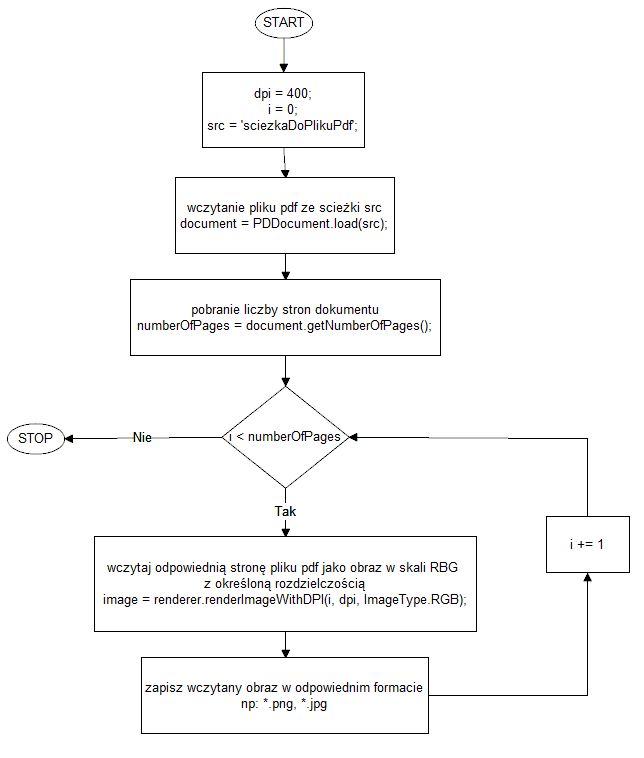
\includegraphics[width=15cm, height=18cm] {image//algorithm//getImgFromPdf.png} 
			\end{center}
			\caption
    			[Algorytm pobierania obrazów z plików pdf]  
	    		{Algorytm pobierania obrazów z plików pdf}  
		\end{figure}
		
		\subsubsection{Klasa ImproveImg}
			\paragraph{} Algorytmy przetawrzające obraz zaimplementowane w klasie           ImproveImg przygotowują go do dalszej obróbki przez 'polepszenie' jego      jakości w tym redukcji szumów, dzięki wykorzystaniu metod rozmycia i        progowania udostępnionych przez bibliotekę OpenCv, które pracują na         obrazie wczytanym w skali szarości.  \par
			
			    \textbf{Rozmycie}
			    Operacja ta nosi również nazwę wygładzania, przyczyny wykonania zabiegu rozmycia na obrazie mogą być różne, w znaczącej wiekszości przypdaków powodem jest chęć usunięcia występujących szumów. Do wyboru( w bibliotece OpenCv) mamy kilka funkcji, posługujących się róznymi rodzajami filtrów dolnoprzepustowych, a więc wykorzystującymi różne jądra, będące de facto współczynnikami tych filtrów. Algorytm wykorzystuje funkcję:
			    \textit{Imgproc.medianBlur(src, dst, ksize);}
			    gdzie \textit{ksize} jest rozmiarem jądra, które jest nieliniowe oraz:  
			    
			    \begin{displaymath}
                    ksize\, \epsilon\, \mathbb{N}\, \wedge\, ksize\, \epsilon\, \mathbb{Z}\, \wedge\, ksize\pmod{2} = 1
                \end{displaymath}
                
                \paragraph{} Filtr ten warość poszczególnych pikseli zmienia na medianę, któa zostaje obliczona uwzględniając wartości pikseli tworzących określony prostokąt w którego centrum jest zmieniany piksel. \par
			     
			    \textbf{Progowanie}
			    Jedną z najprostszych metod segmentacji obrazu jest operacja progowania.  Biblioteka udostpnia dwa warianty progowań: proste i adaptacyjne. 
			    Wśród progowań prostych możemy wybrać jedną z następujących możliwości( \textit{thresholdType}): BINARY, BINARY\_INV, TRUNC, TOZERO, TOZERO\_INV.
			    Algorytm wykorzystuje proste progowanie binarne( BINARY), które wartość każdego z pikseli obrazu( \textit{src}) porównuje z zadanym progiem( \textit{threshold}) i jeśli jego wartość jest od niego większa to, temu pikselowi przypisywana jest wartość \textit{maxValue}, następnie obraz zapisywany jest w nowej macierzy( \textit{dst}).\\
			    \textit{Imgproc.threshold(src, dst, threshold, maxValue, thresholdType//*Imgproc.THRESH\_BINARY*//);}
			    
			    \begin{displaymath}
                    dst( x, y) =  
                    \left\{
                        \begin{array}{ll}
                            maxValue & \textrm{dla } src( x, y) > threshold \\
                            0 & \textrm{dla } src( x, y) \leqslant threshold
                        \end{array}
                    \right.
                \end{displaymath}
			    
			    \newpage
    		    
    		    \begin{figure}[!ht]  
    			    \begin{center}
    				    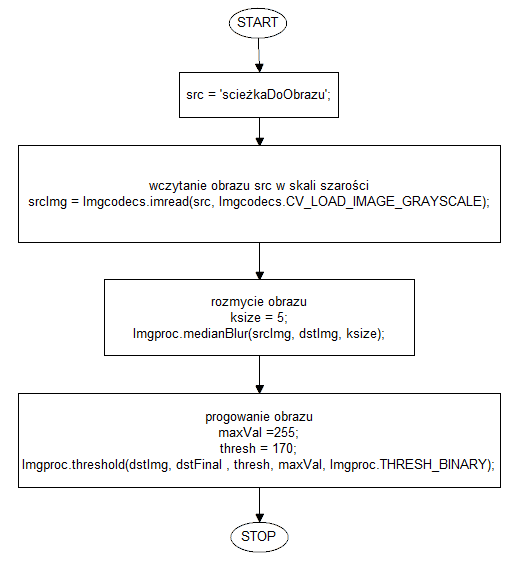
\includegraphics[width=12cm, height=12cm] {image//algorithm//improveImg.png} 
    			    \end{center}
    			    \caption
        			    [Algorytm polepszenia jakości obrazów]  
	    		        {Algorytm polepszenia jakości obrazów}  
    		    \end{figure}
		
%		\setcounter{figure}{0} 
%		\renewcommand{\figurename}{Zdjęcie.}
		
    		    \begin{figure}[!ht]  
    			    \begin{center}
    				    \includegraphics[height=8.5cm, frame] {image//exampleImage//001_a.jpg} 
    			    \end{center}
    			    \caption
        			    [Obraz przed zastosoawaniem algorytmu]  
                        {Obraz przed zastosoawaniem algorytmu}  
    		    \end{figure}
		
		        \begin{figure}[!ht]  
    			    \begin{center}
    				    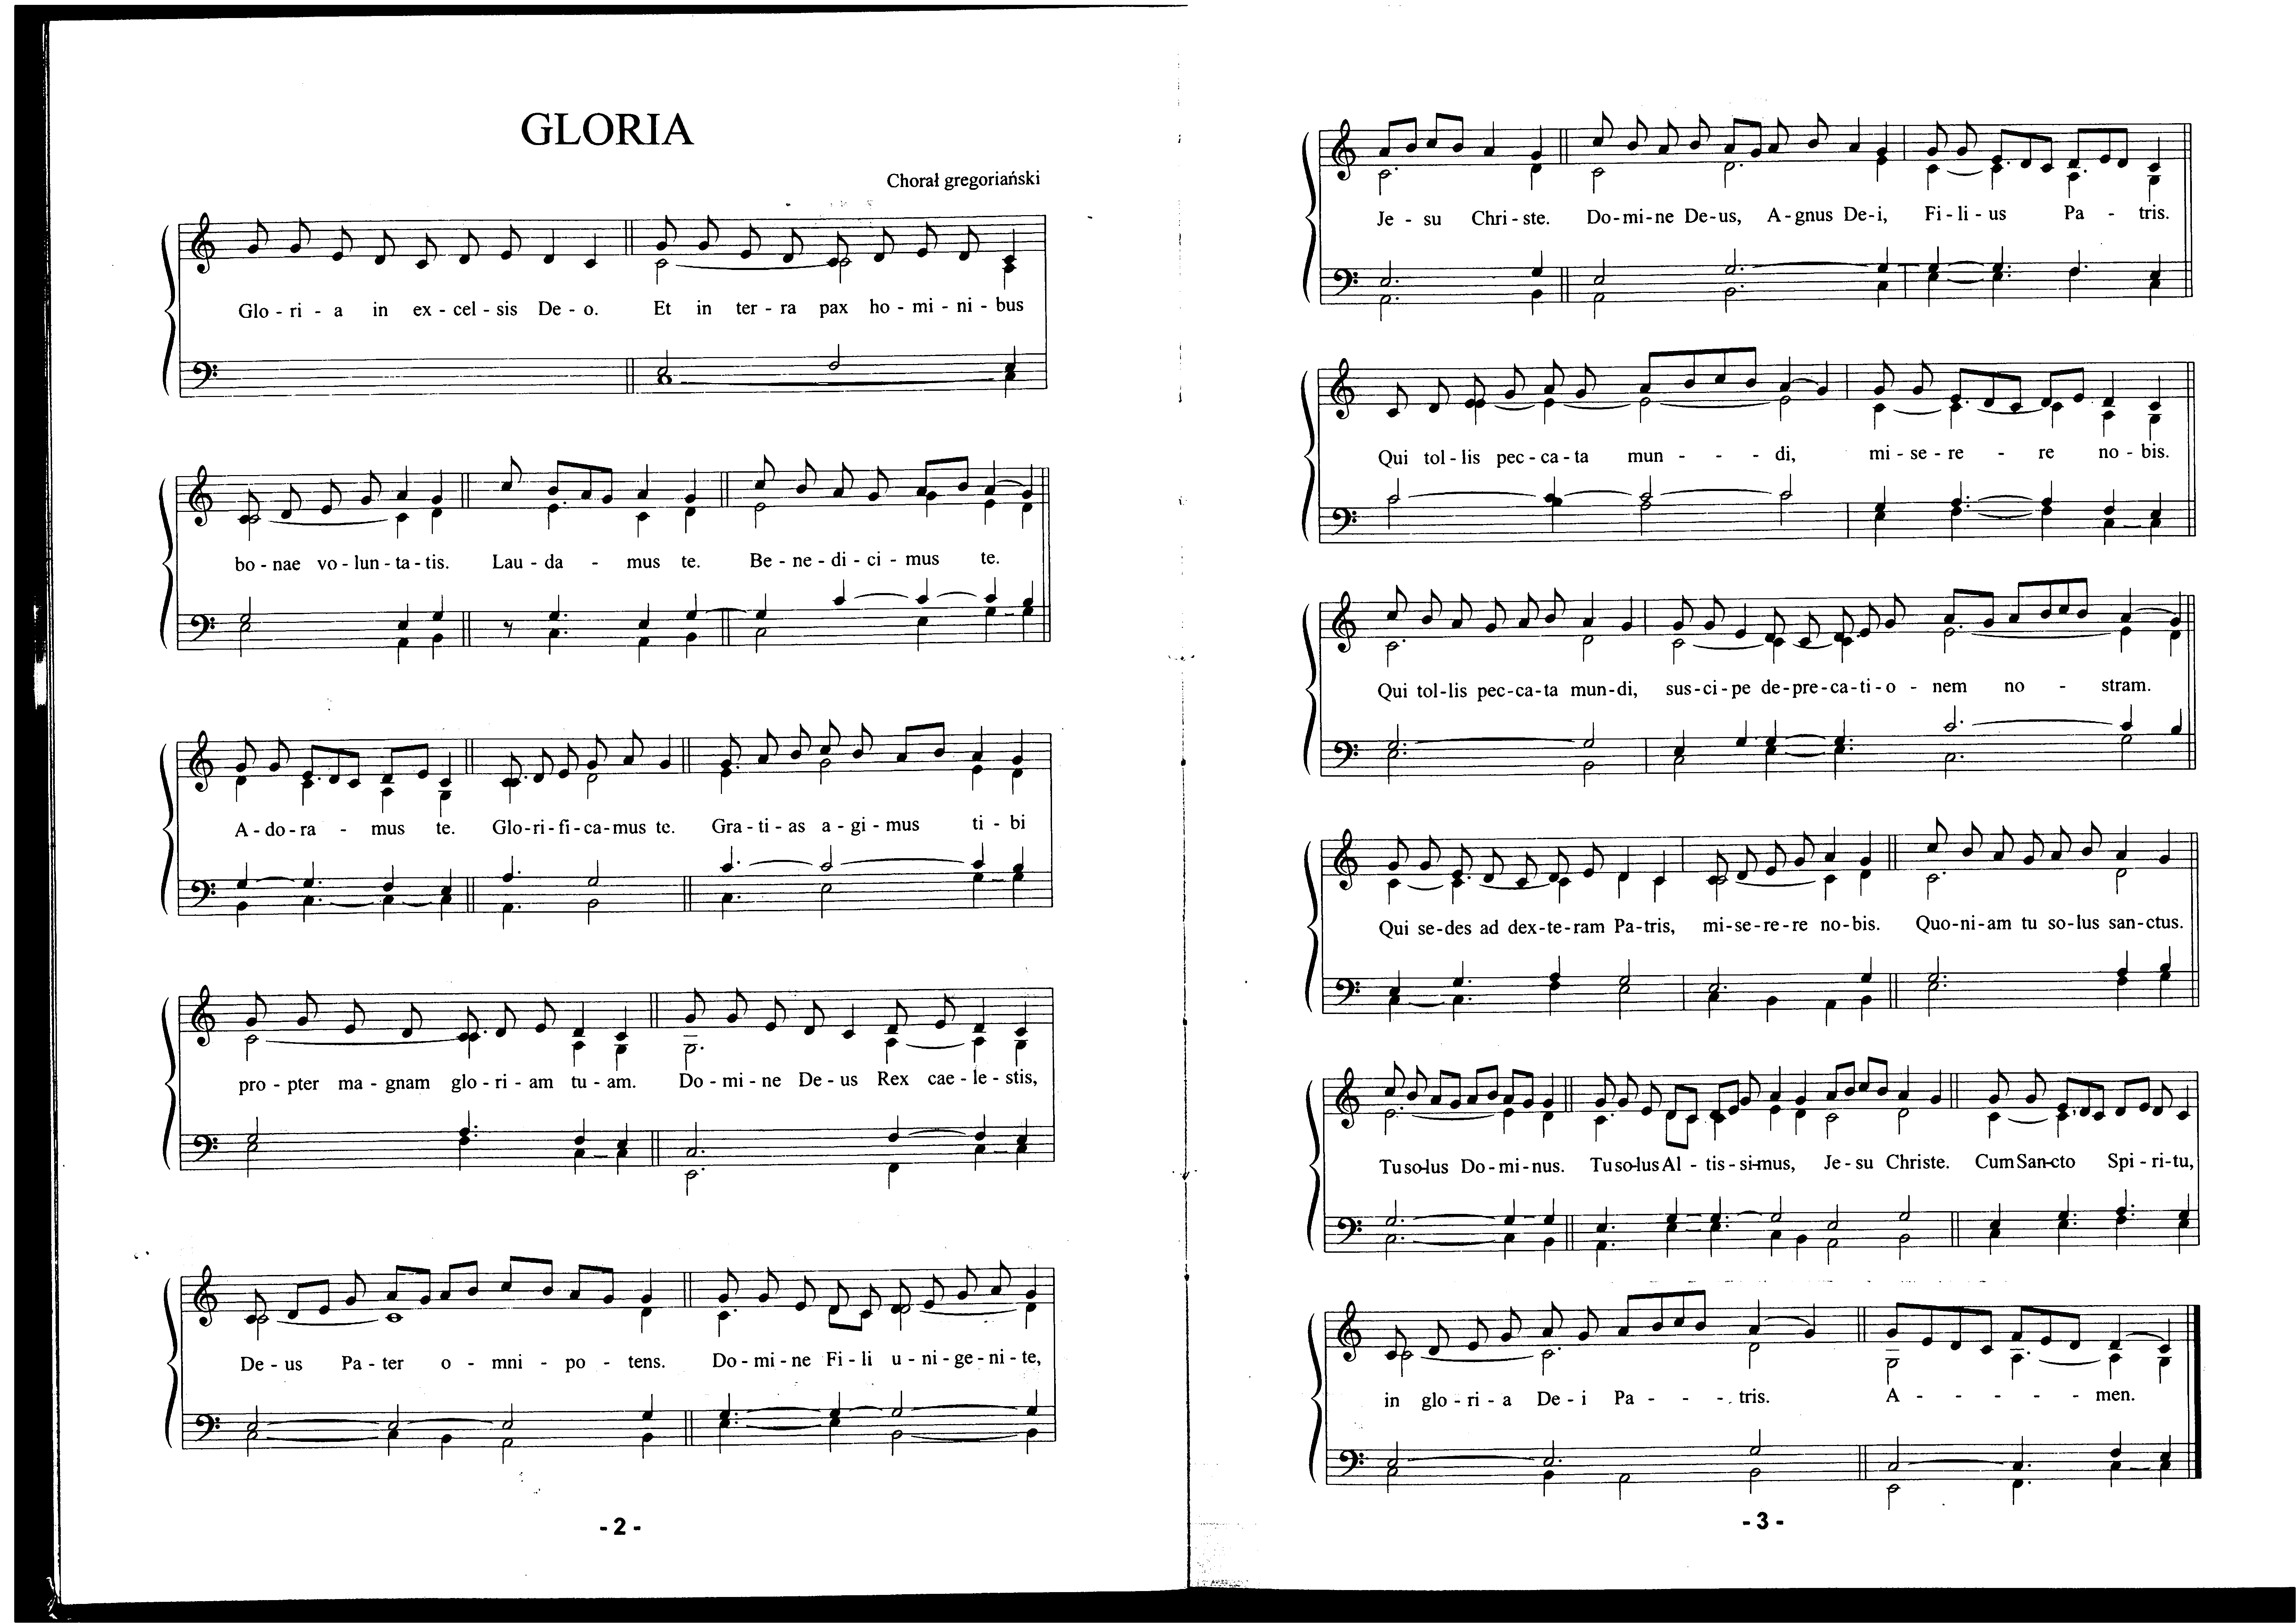
\includegraphics[height=8.5cm, frame] {image//exampleImage//001_b.png} 
    			    \end{center}
	    		    \caption
    			        [Obraz po zastosowaniu algorytmu polepszającego jego jakość]  
	    		        {Obraz po zastosowaniu algorytmu polepszającego jego jakość}  
	            \end{figure}
		
		\subsubsection{Klasa CutBlackArea}
			\paragraph{} Metody zaimplementowane w klasie umożliwiają wycięcie z obrazu     czarnych obszarów, które są uzupe\l nieniem interesujących nas zakresów     stron do określonego formatu skanu. Algorytm wykorzystuje do tego           wartości odchylenia standardowego w poziomych liniach obrazu i wartości     dominanty. Przy założeniu, że te powierzchnie znajdują się po lewej         stronie i na dole obrazu. Algorytm umożliwia wycięcie jednego( dolnego)     lub obu obszarów. 
			
    			\begin{figure}[!ht]  
    			    \begin{center}
    				    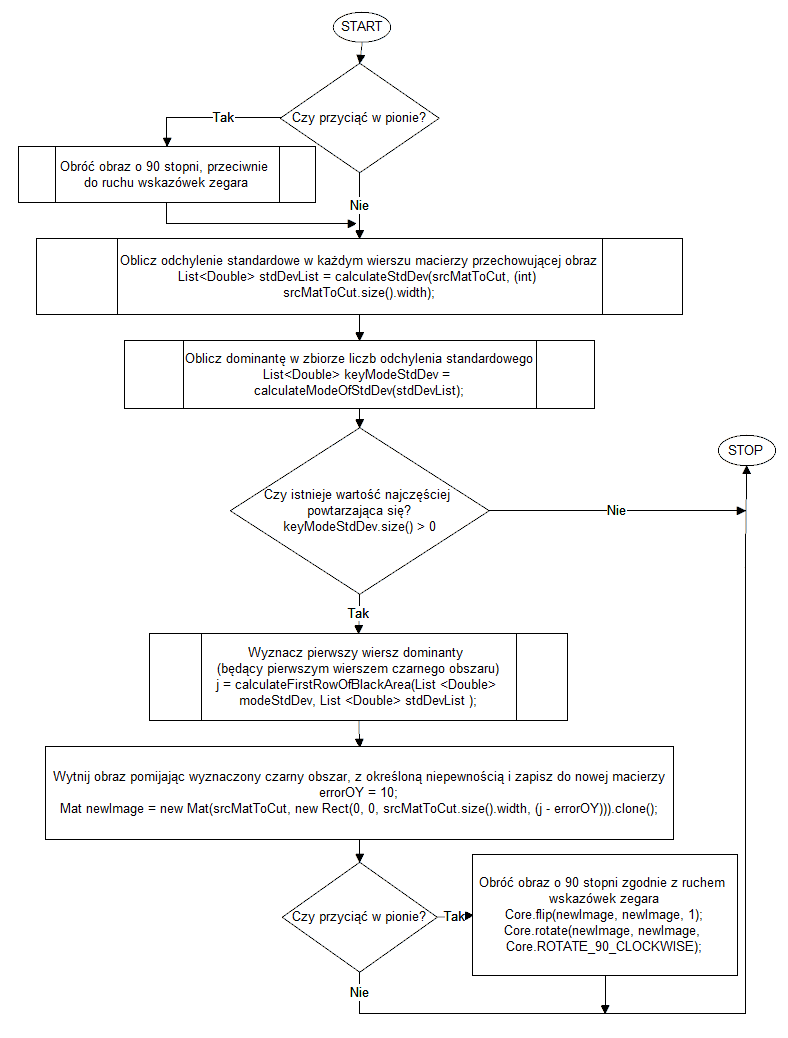
\includegraphics[height=15cm, width=12cm] {image//algorithm//cutBlackArea.png} 
    			    \end{center}
    			    \caption
        			[Algorytm usuwający czane obszary z obrazu]  
    	    		{Algorytm usuwający czane obszary z obrazu}  
    		    \end{figure}
		    
		        \newpage
		    
    		    \begin{figure}[!ht]  
    			    \begin{center}
    				    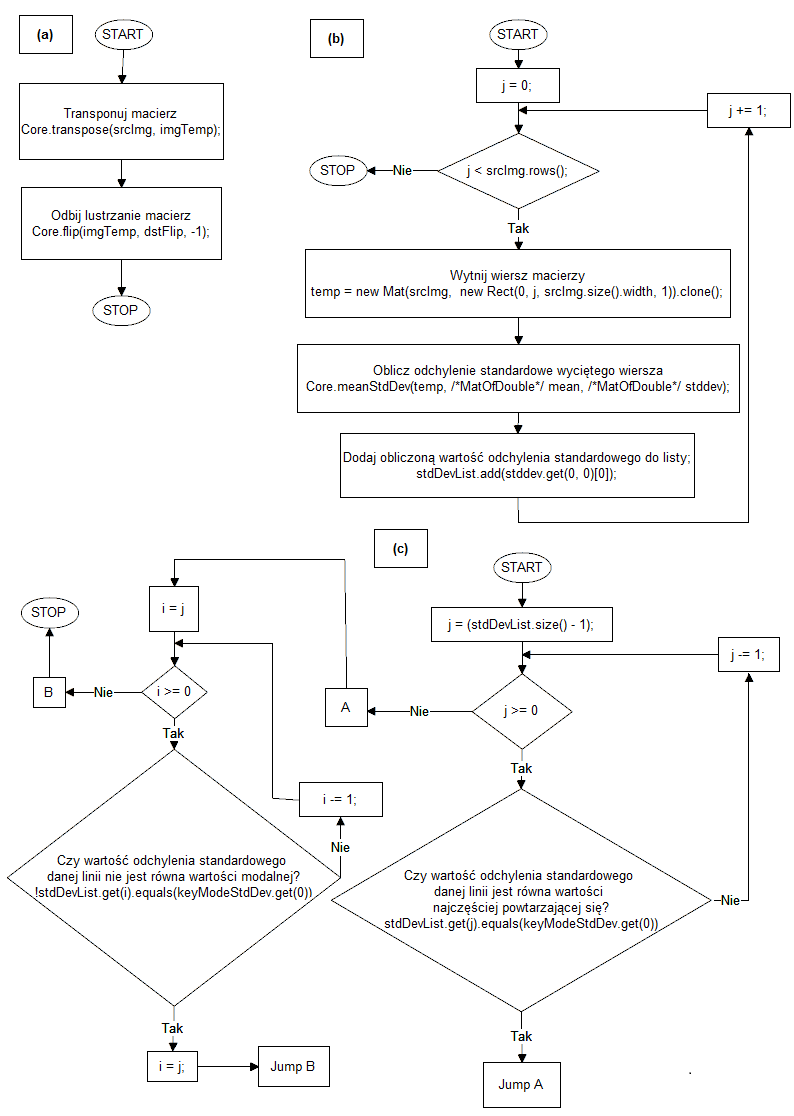
\includegraphics[height=22cm, width=17cm] {image//algorithm//cutBlackAreaPred.png} 
    			    \end{center}
    			    \caption
            			[Poszczególne funkcje algorytmu a) Obrót o 90 stopni zgodnie z ruchem wskazówek zegara, b)Obliczenie odchylenia standardowego wierszy macierzy, c) Wykrycie wycinanego( czarnego) obszaru]  
        	    		{Poszczególne funkcje algorytmu a) Obrót o 90 stopni zgodnie z ruchem wskazówek zegara, b)Obliczenie odchylenia standardowego wierszy macierzy, c) Wykrycie wycinanego( czarnego) obszaru}
    		    \end{figure}
			    
			    \guilsinglleft
			
			    \newpage
	        
	            \begin{figure}[!ht]  
		            \begin{center}
			            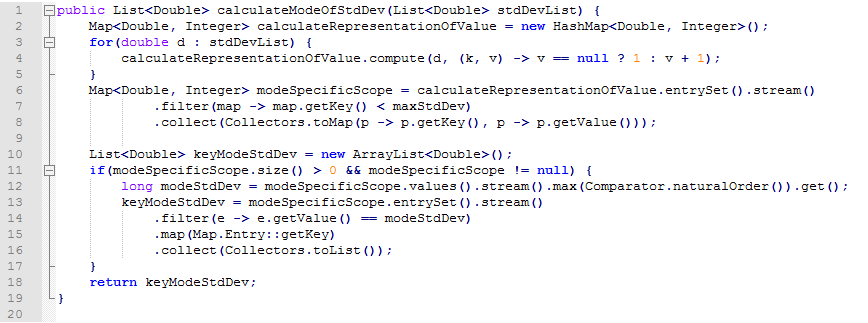
\includegraphics[width=17cm, frame] {image//algorithm//modeAlgorithm.png} 
		            \end{center}
			        \caption
    			        [Kod funkcji obliczajacej dominantę]
    			        {Kod funkcji obliczajacej dominantę}  
		        \end{figure}
			
    			\begin{figure}[!ht]  
    			    \begin{center}
    				    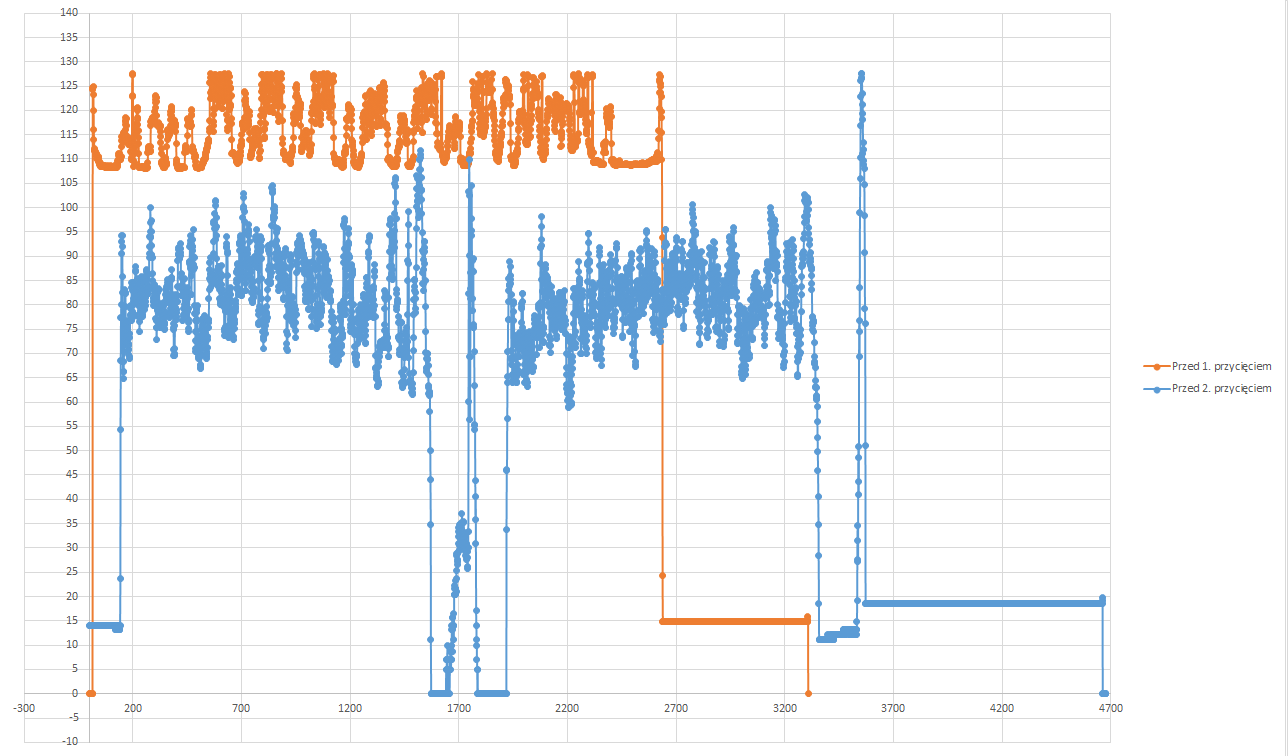
\includegraphics[width=17cm, height=8cm, frame] {image//practicalPart//stdDevCutBlackArea.png} 
    			    \end{center}
    			    \caption
            			[Odchylenie standardowe w funkcji wieszy macierzy] 
            			{Odchylenie standardowe w funkcji wieszy macierzy}  
    		    \end{figure}
			
    			Na podstawie wykresu widzimy, że wiersze obrazu( w skali szarości) o ma\l ej zmienności wartości pikseli, będą dawa\l y niewielkie wartości odchylenia standardwego. Jeśli nie równa się ono zeru, ale jest odpowiednio ma\l e możemy za\l ożyć, że badany wiersz ma jedną barwę, a wartość ta wynika z drobnych zak\l uceń i niedoskona\l ości obrazu.
    			
    			Do obliczenia odchylenia standardowego została użyta funkcja udostępniona w bibliotece OpenCv:\textit {Core.meanStdDev(Mat src, MatOfDouble mean, MatOfDouble stddev)}. Oblicza ona średnią i odchylenie standardowe macierzy podanej jako parametr src( w algorytnie jest to jeden wiersz obrazu), które zależy od wszystkich kanałów macierzy. Tutaj jest to jeden kanał --- obraz przed obliczeniami został prztransformowany do skali szarości według poniższego algorytmu:
    			 		
    			Za obliczenie wartości najczęściej występującej odchylenia standardowego odpowiada funkcja: \textit {public List \guilsinglleft Double\guilsinglright calculateModeOfStdDev(List \guilsinglleft Double\guilsinglright stdDevList)}
    			wykorzystująca nowe rozwiązania wprowadzone w Javie wersji 8, a więc strumienie i wyrażenia lambda, co znacząco przyśpiesza czas obliczeń oraz przejrzystość napisanego kodu.  
			
			
    		    \begin{figure}[!ht]  
    			    \begin{center}
    				    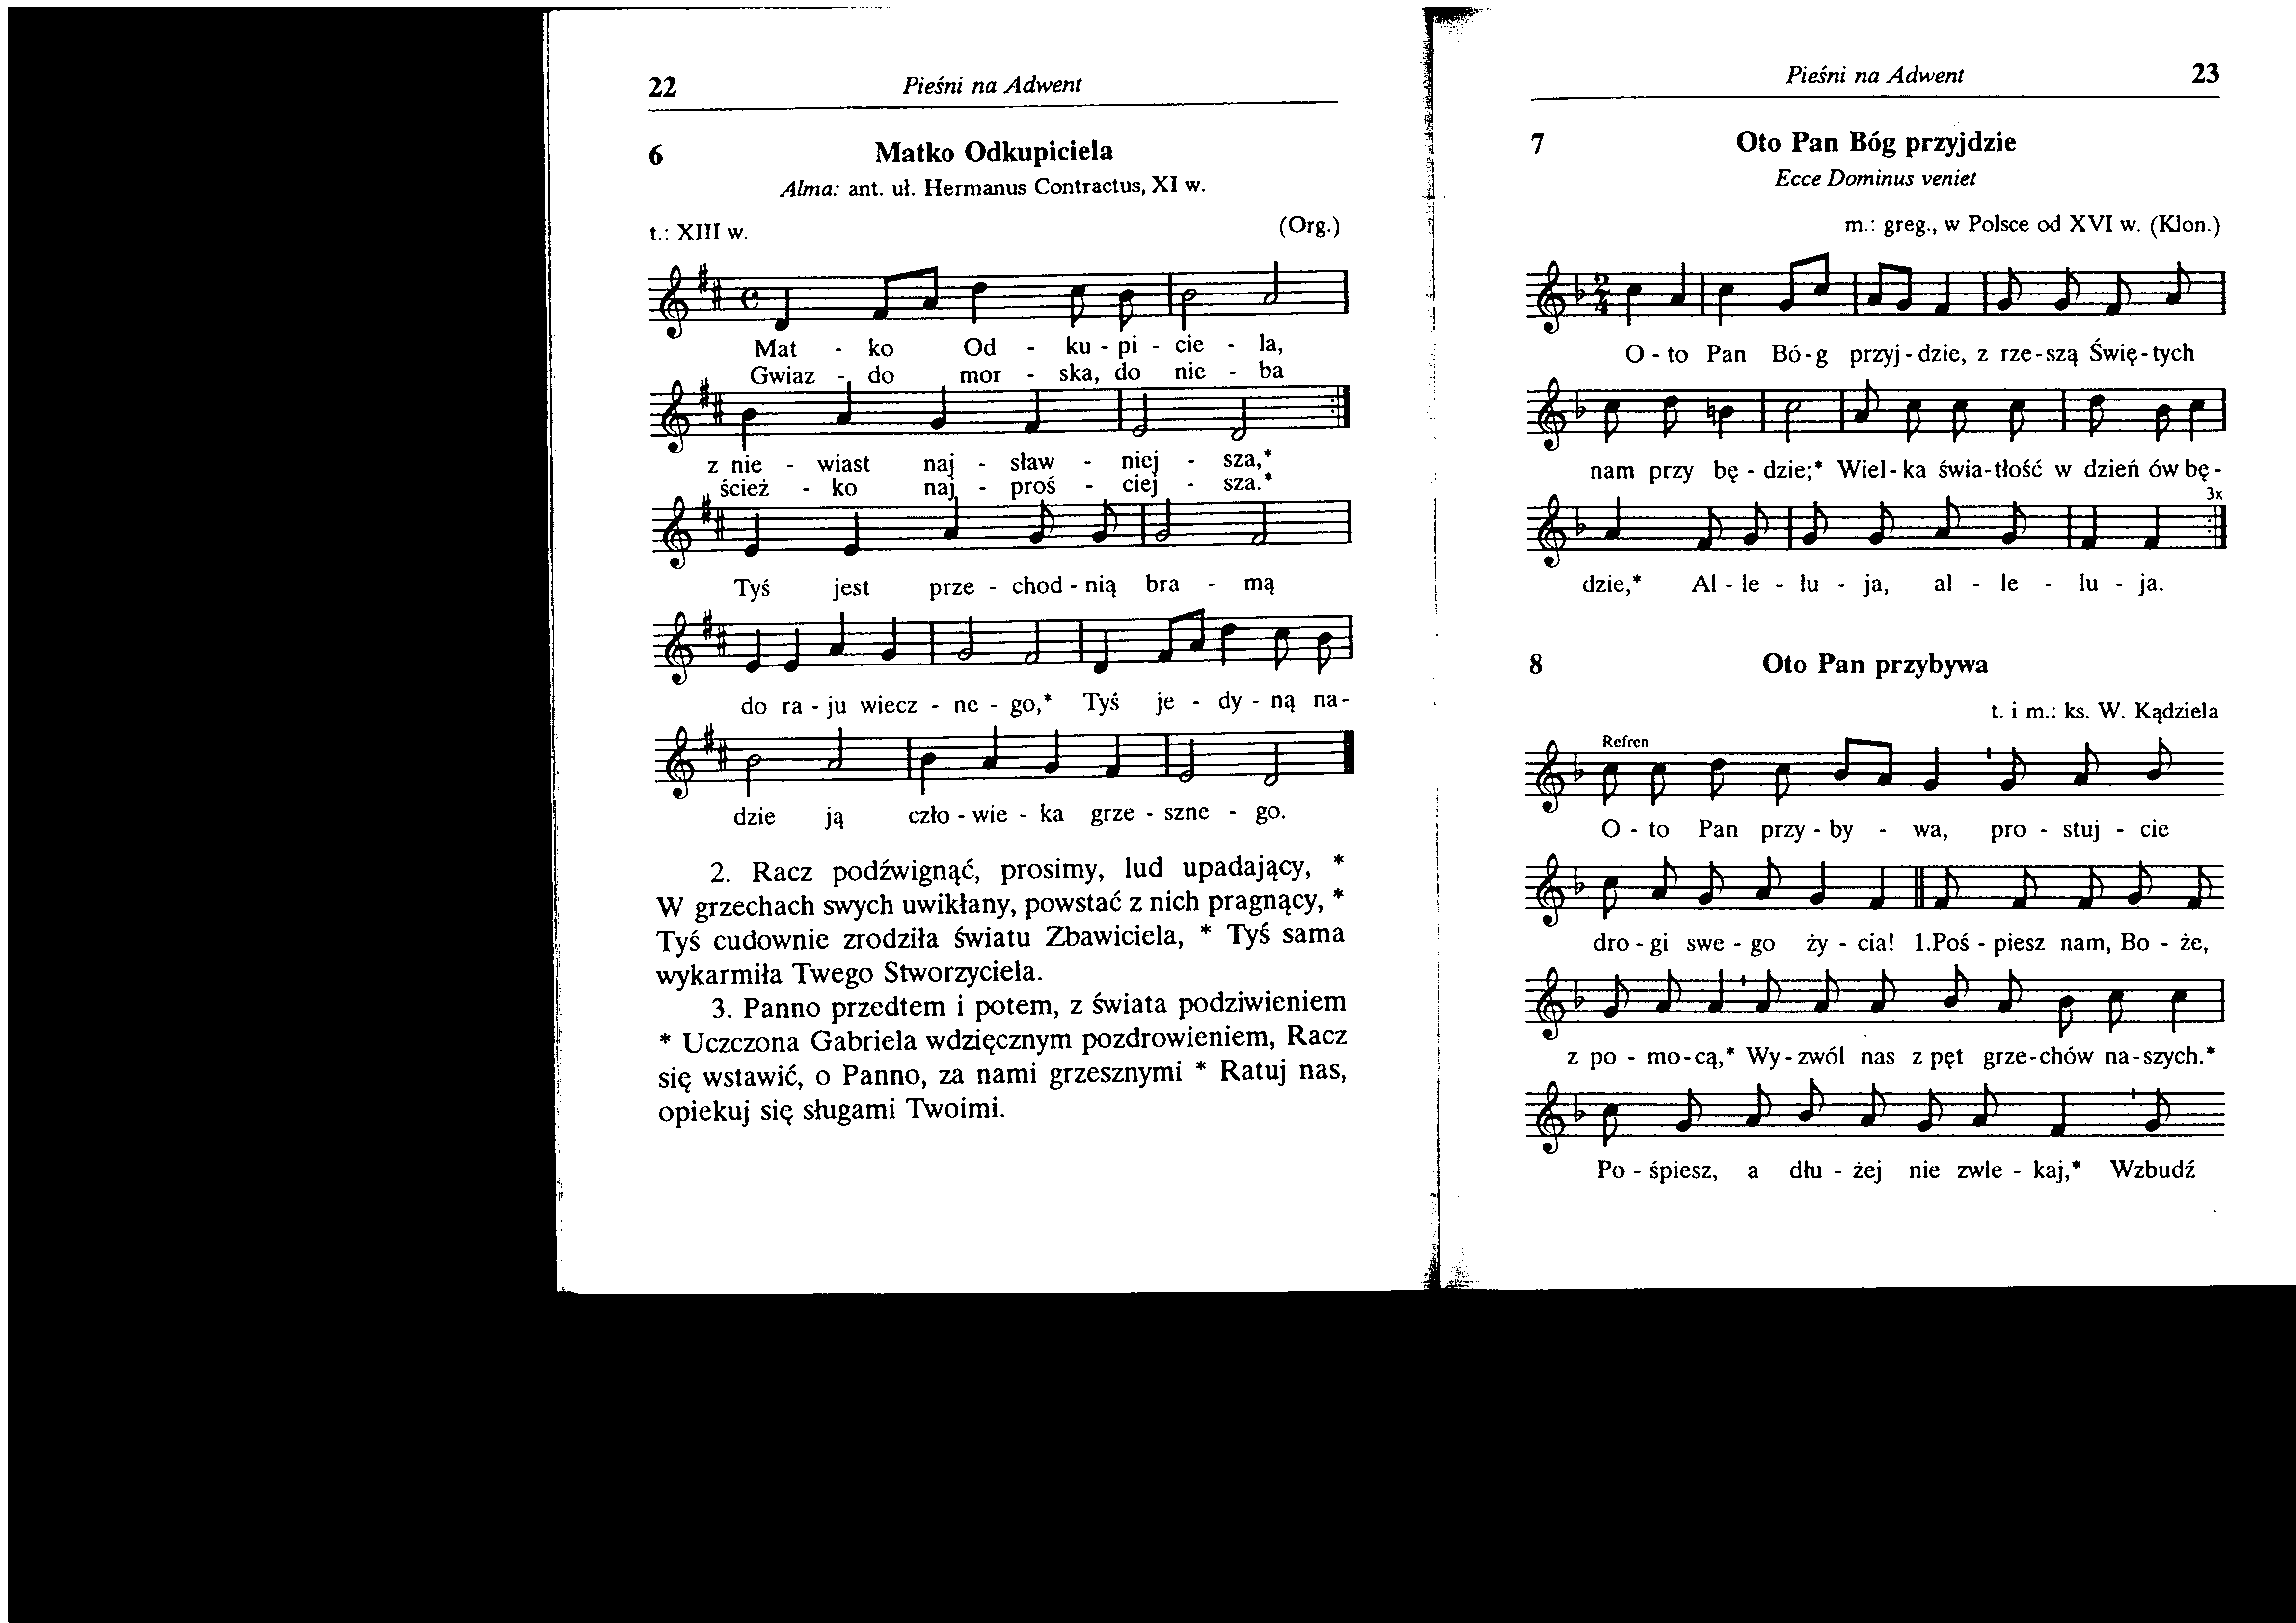
\includegraphics[height=8.25cm, frame] {image//exampleImage//002_a.png} 
    			    \end{center}
    			    \caption
    			        [Obraz przed usunięciem nadmiarowych obszarów]
        			    {Obraz przed usunięciem nadmiarowych obszarów}  
    		    \end{figure}
    		    
    		    \begin{figure}[!ht]  
    			    \begin{center}
    				    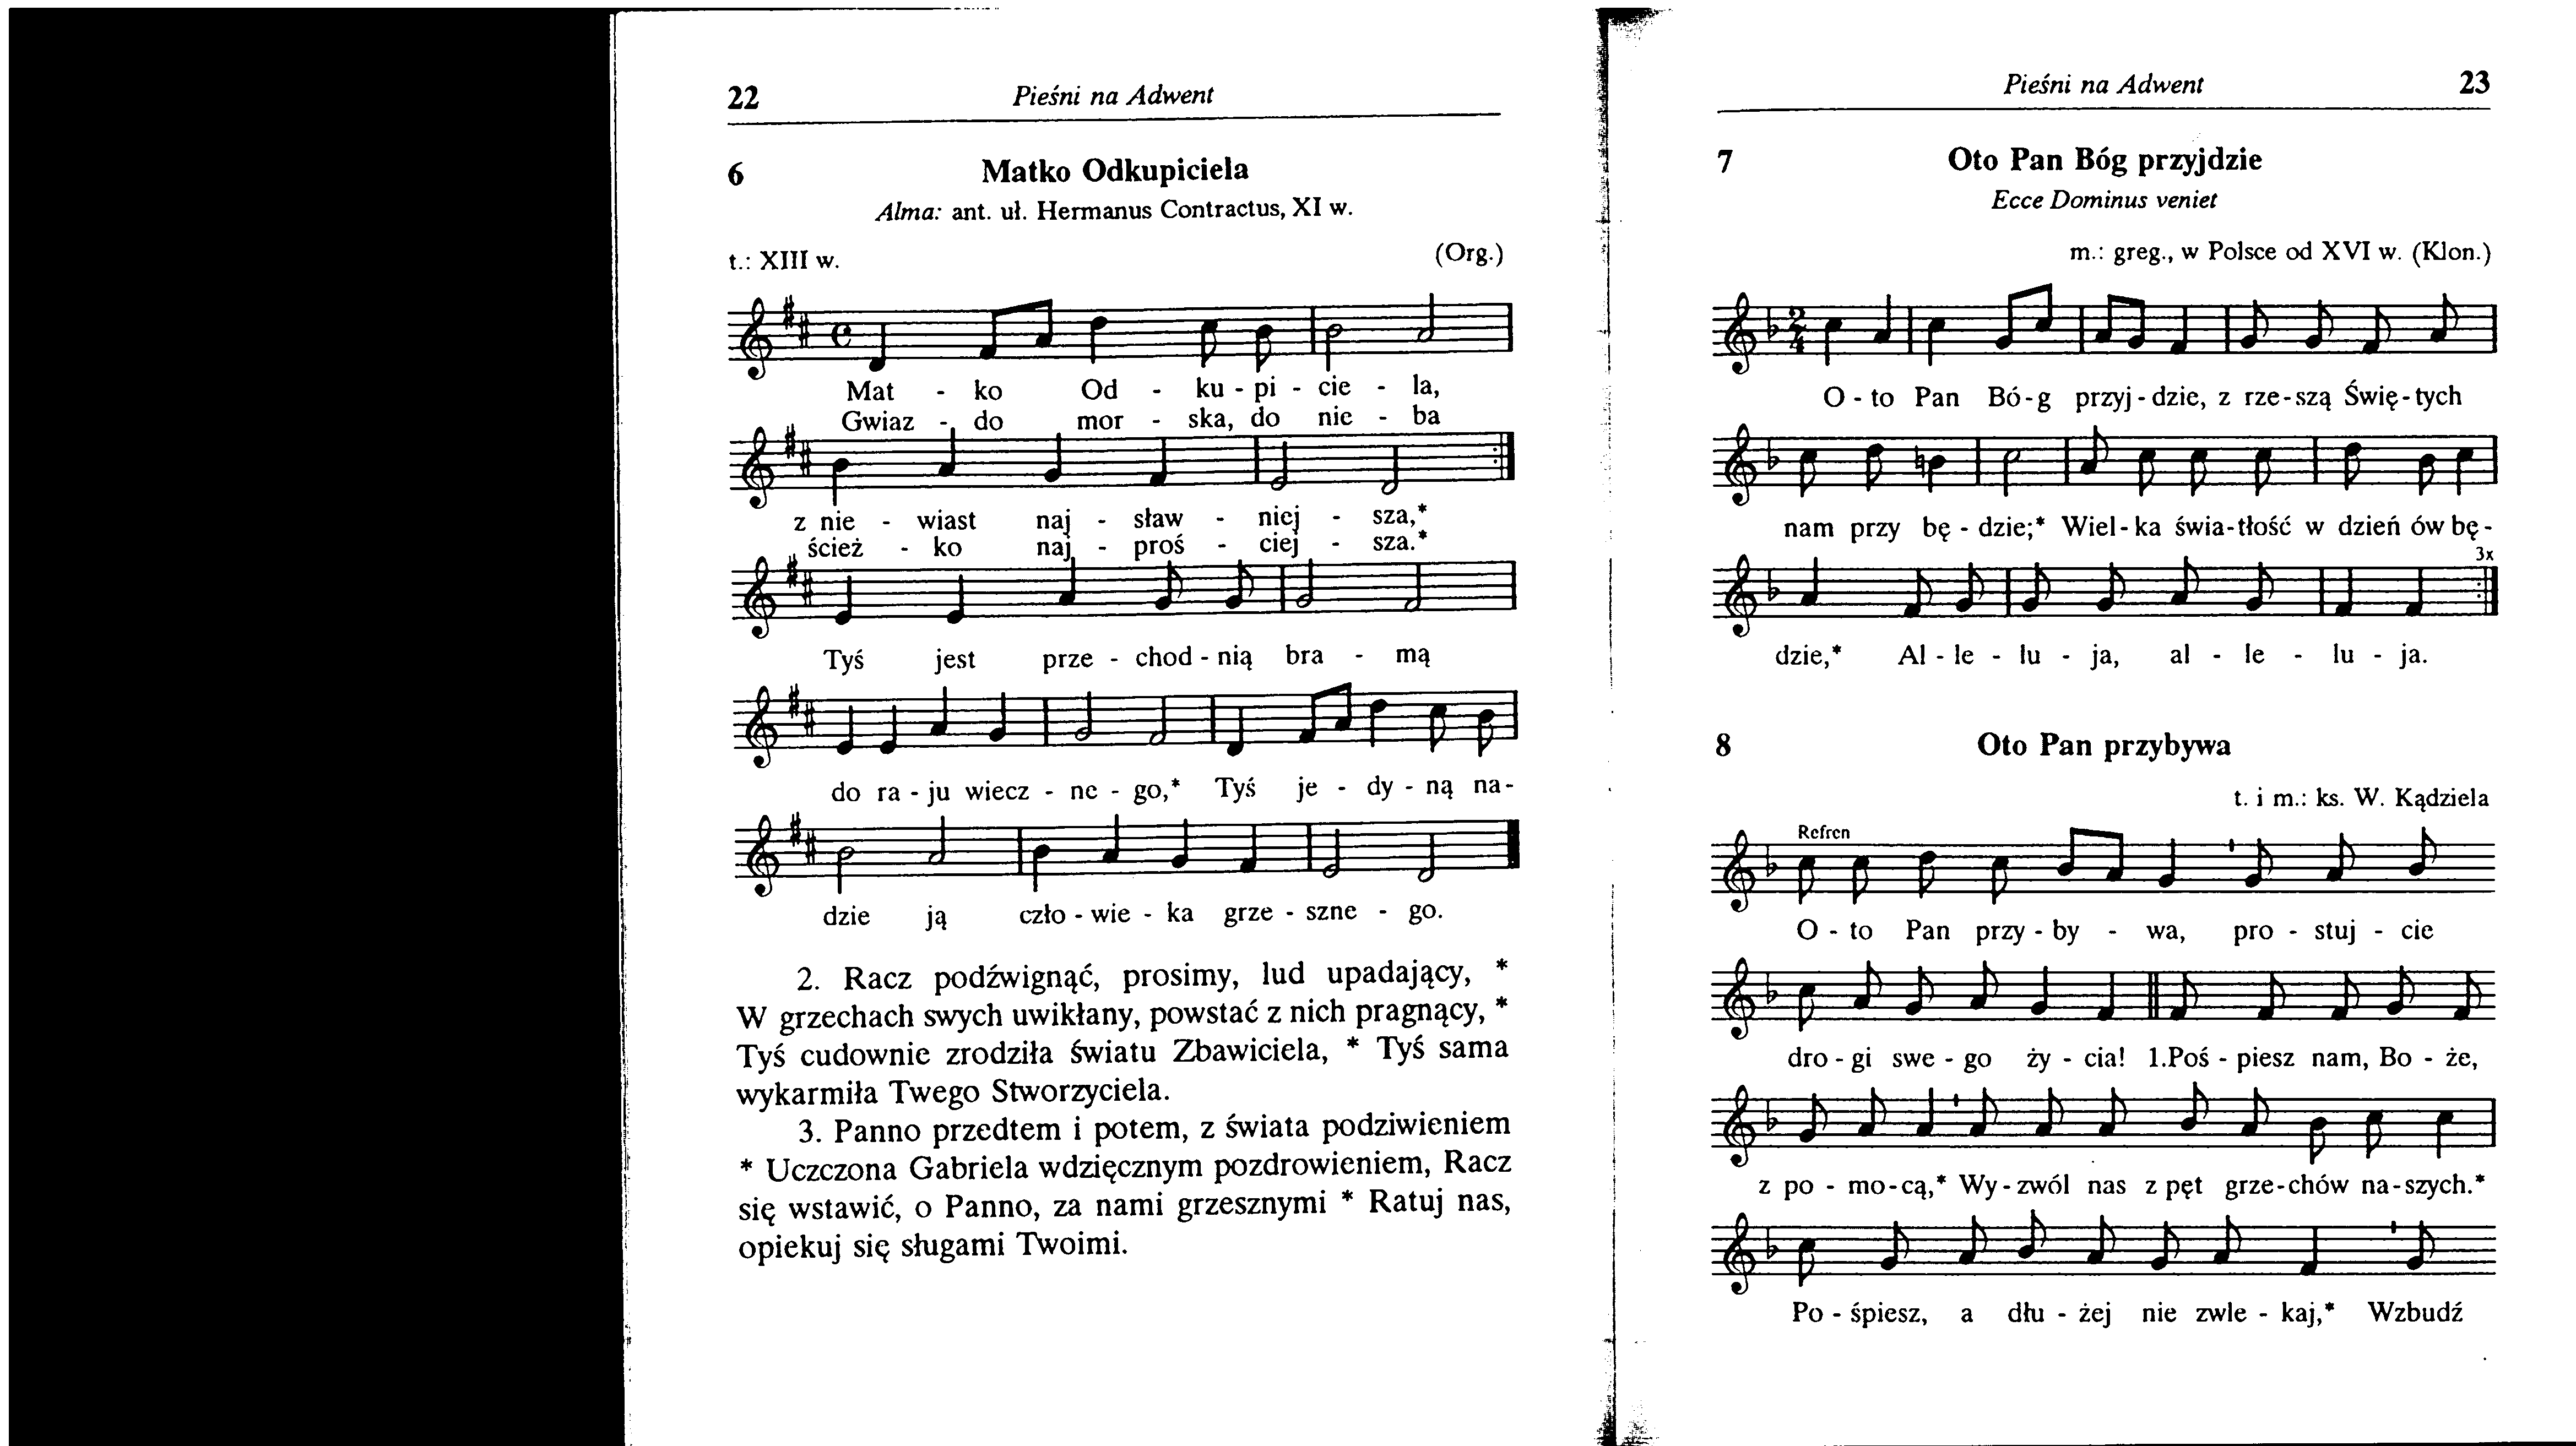
\includegraphics[height=8cm, frame]{image//exampleImage//002_b.png} 
    			    \end{center}
    			    \caption
            			[Obraz po przycięciu obszaru znajdującego się na dole]  
        			    {Obraz po przycięciu obszaru znajdującego się na dole}  
    		    \end{figure}
    			
    	        \begin{figure}[!ht]  
    			    \begin{center}
    				    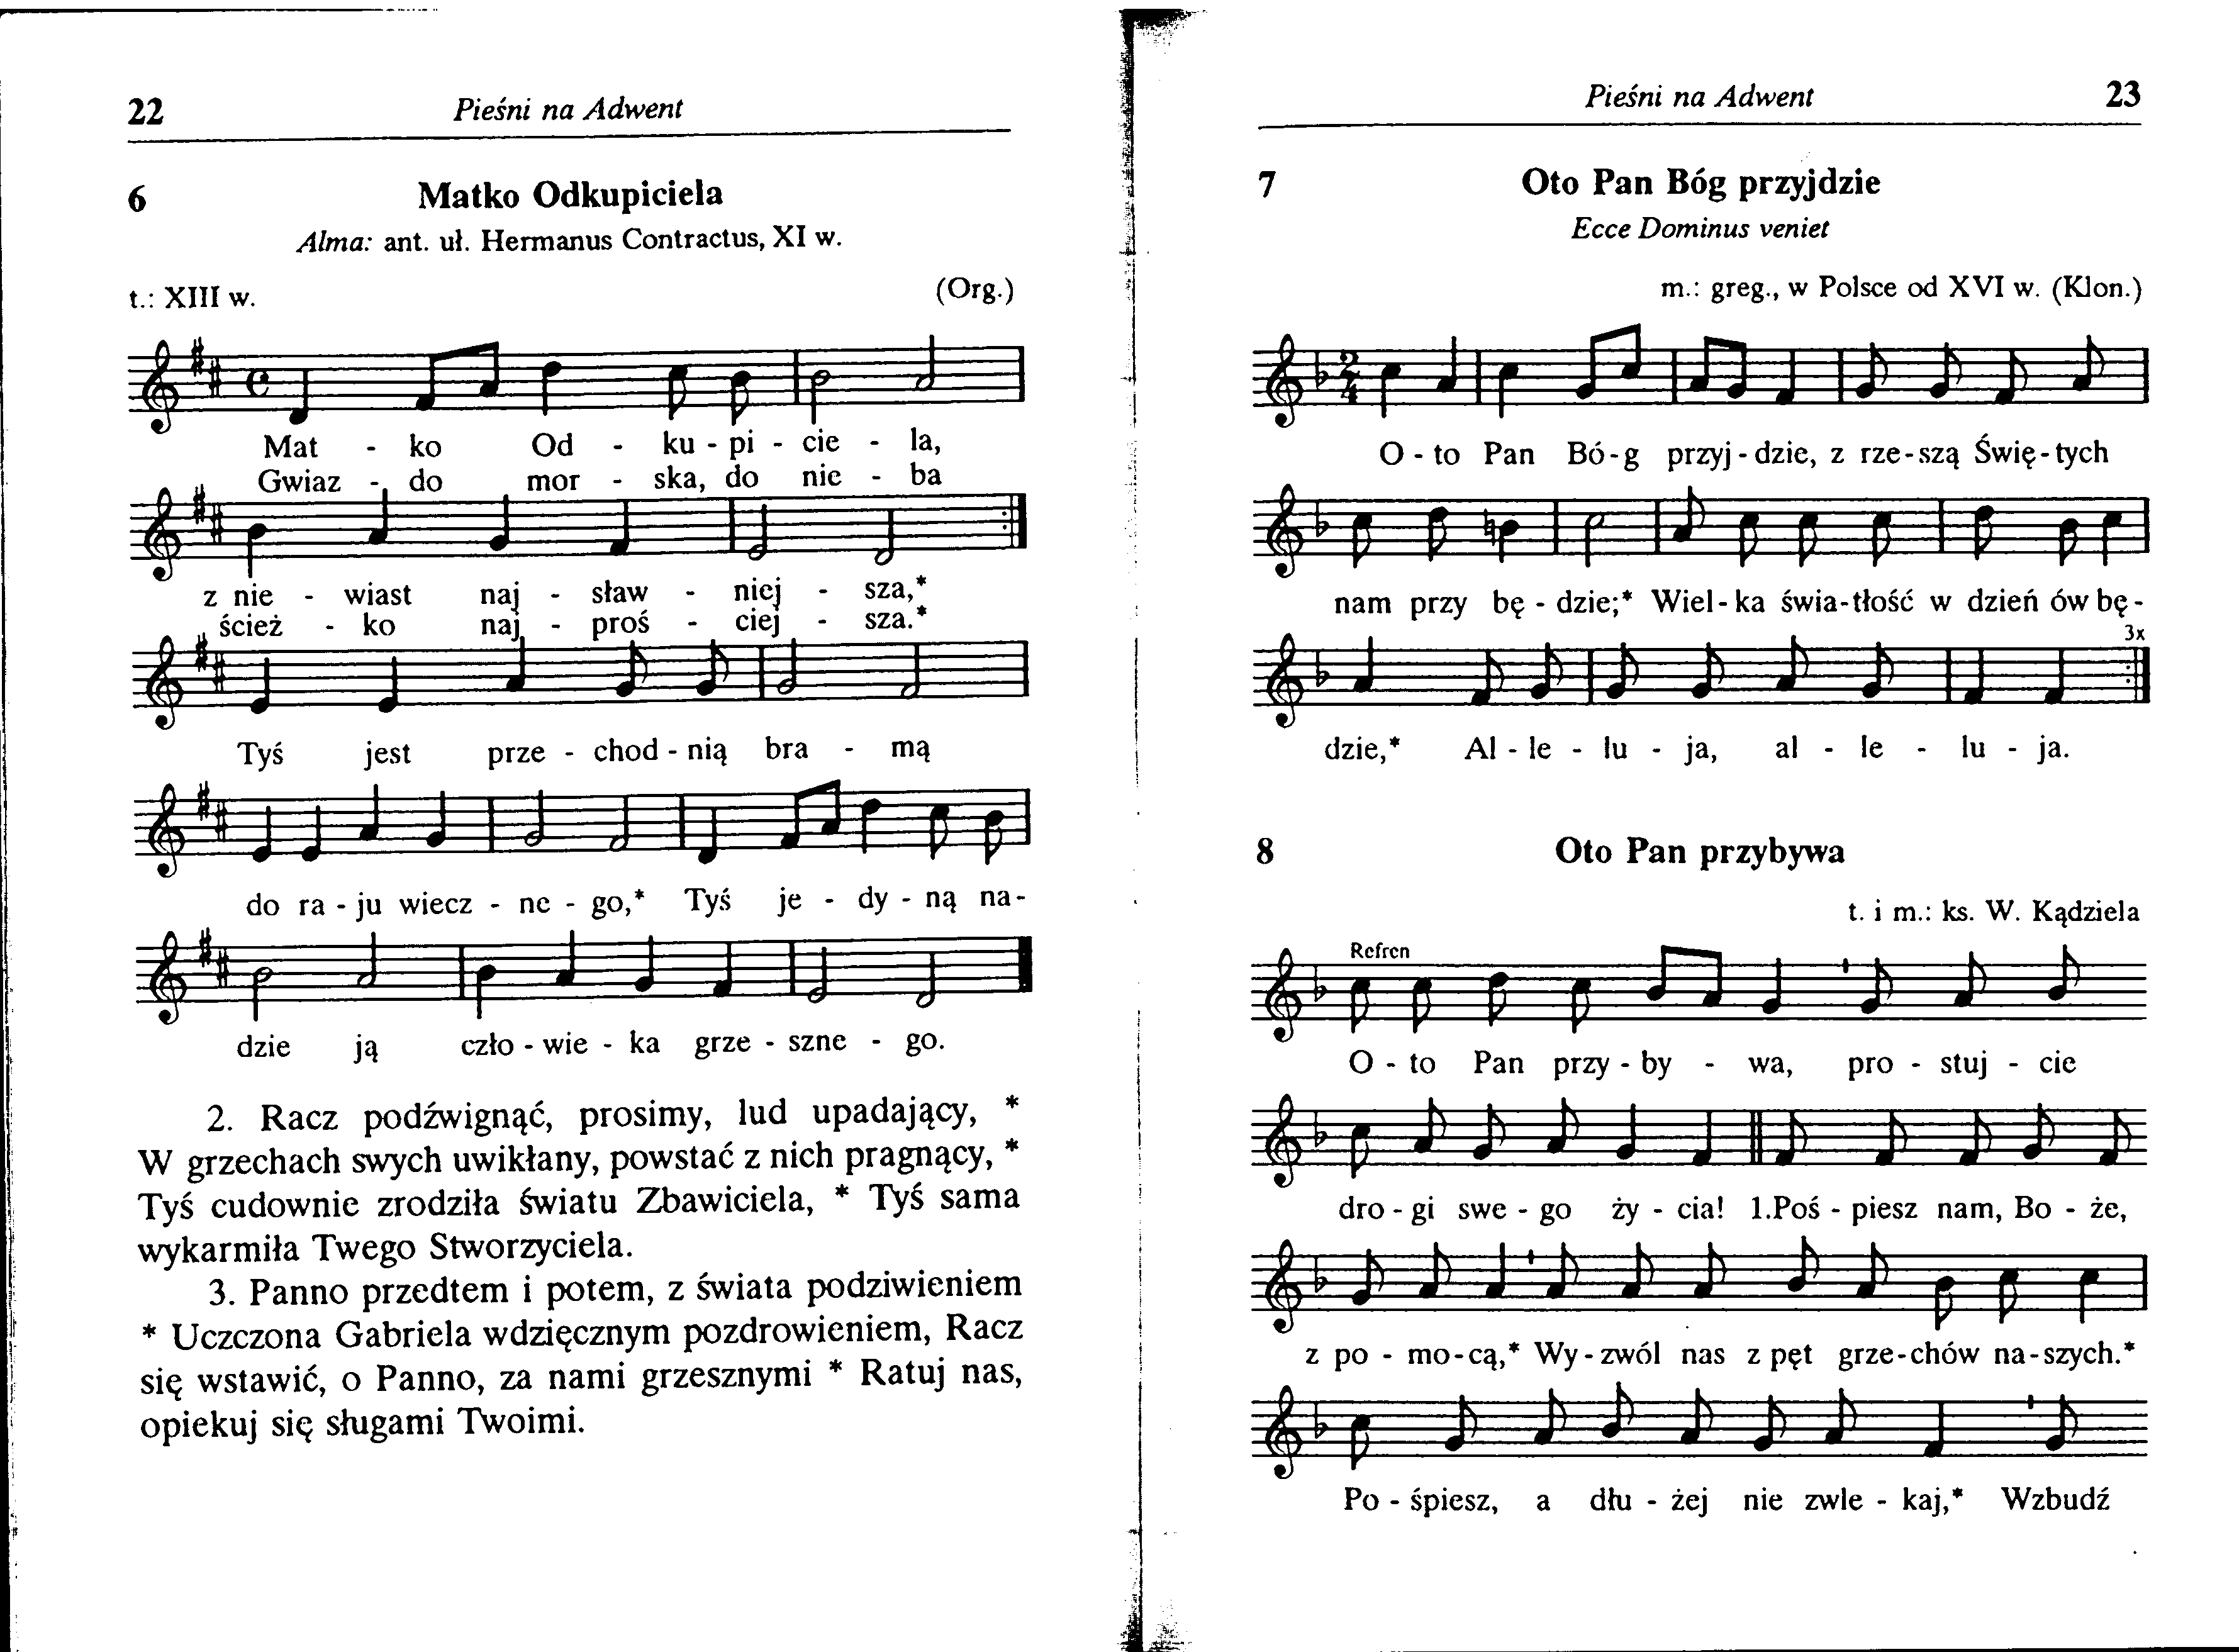
\includegraphics[height=8cm, frame] {image//exampleImage//002_c.png}
    			    \end{center}
        			\caption
        			    [Obraz po przycięciu obszaru znajdującego się po lewej stronie]
        			    {Obraz po przycięciu obszaru znajdującego się po lewej stronie} 
    		    \end{figure}
			
		\subsubsection{Klasa DivideToPage}
		    \paragraph{} Wykorzystanie metod tej klasy umożliwia podzia\l obrazu            zawierającego dwie strony śpiewnika na dwa osobne obraz, z których każdy     stanowi jedną stronę. Algorytm wykorzystuje do tego niedoskonałość          skanu, który w książkach szczególnie tych o znacznej liczbie stron          odciska na ich \l ączeniu charakterystyczny czarny lub zaciemniony          obszar pionowy. Jeżeli wykrycie tego obszaru nie jest możliwe( niewielka     liczba przypadków) przyjęto założenie, że na ca\l y obszar obrazu           przypadają dwie strony śpiewnika i następnie zostaje on podzielony na       dwie części gdzie granicą jest środkowa kolumna macierzy przechowującej     obraz.    
		    
    	        \begin{figure}[!ht]  
    			    \begin{center}
    				    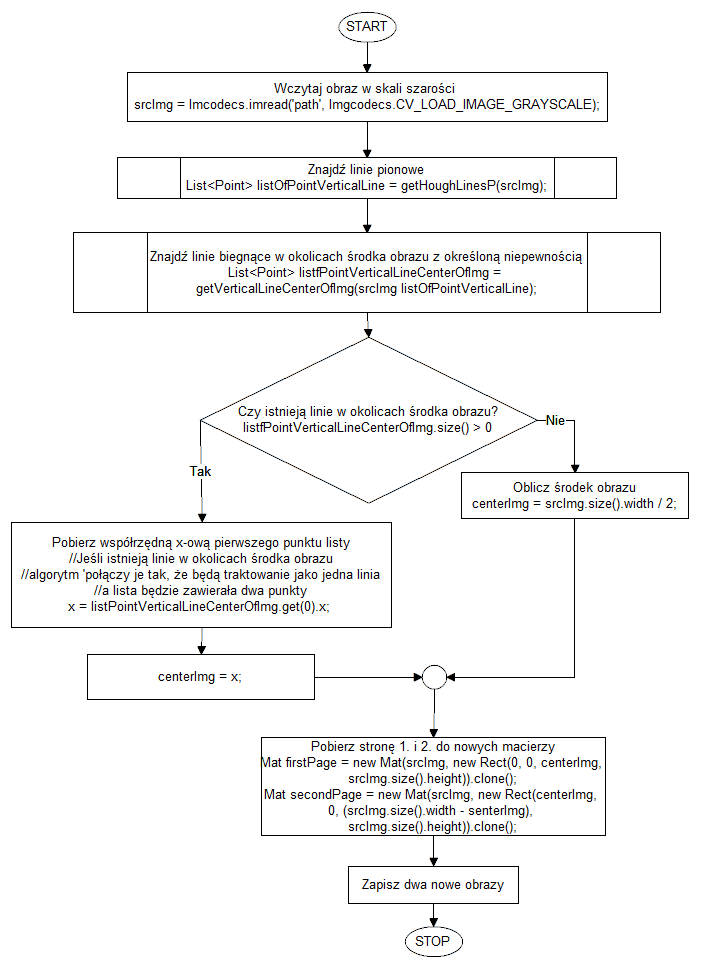
\includegraphics[height=12cm, width=12cm]{image//algorithm//divideToPage.png} 
    			    \end{center}
    			    \caption
        			    [Algorytm dzielący obraz na dwie części, strony]
        			    {Algorytm dzielący obraz na dwie części, strony}  
    		    \end{figure}
    		
    	        \begin{figure}[!ht]  
    			    \begin{center}
    				    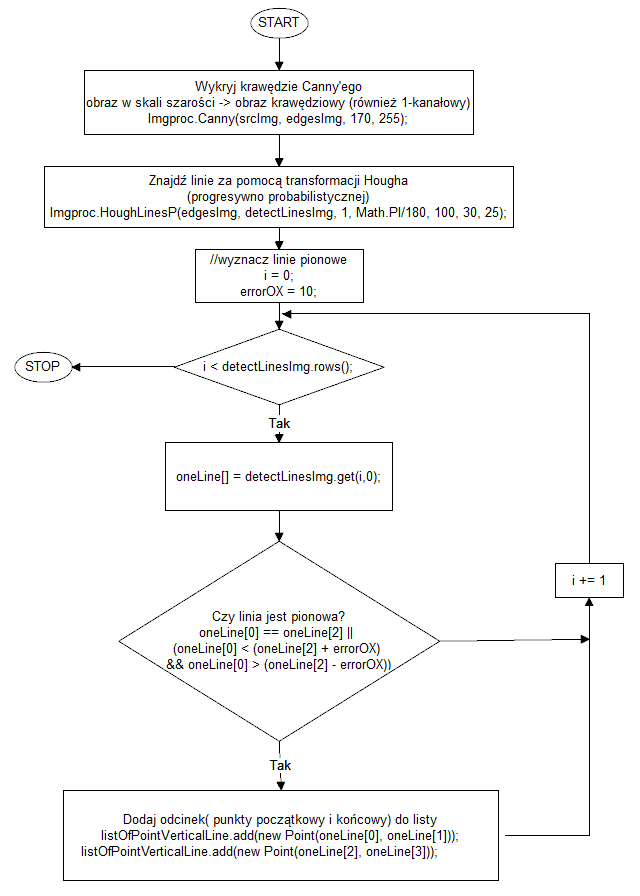
\includegraphics[height=8.5cm, width=8cm]{image//algorithm//divideToPagePred_01.png} 
    			    \end{center}
    			    \caption
        			    [Algorytm znajdujący linie pionowe]  
        			    {Algorytm znajdujący linie pionowe}  
    		    \end{figure}
		
    	        \begin{figure}[!ht]  
    			    \begin{center}
    				    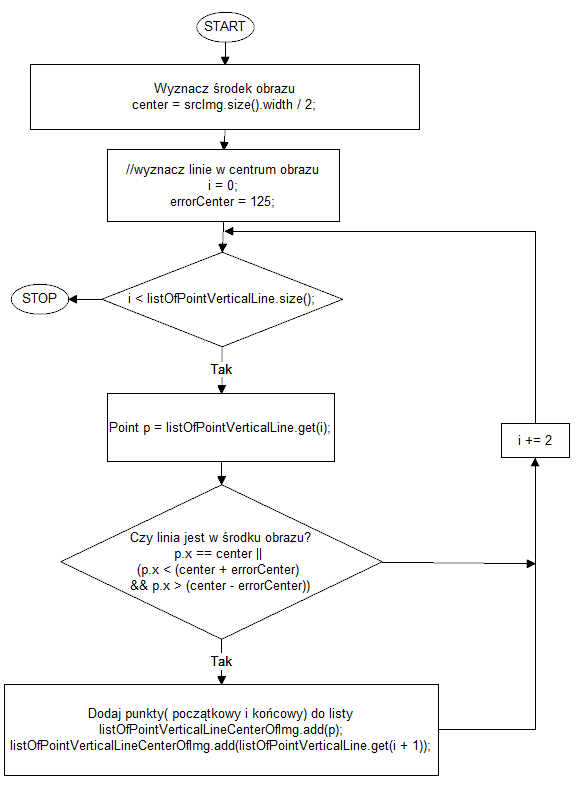
\includegraphics[height=8.25cm, width=8cm]{image//algorithm//divideToPagePred_02.png} 
    			    \end{center}
    			    \caption
        			[Algorytm znajdujący linie pionowe w okolicach środka obrazu]  
        			{Algorytm znajdujący linie pionowe w okolicach środka obrazu}  
    		    \end{figure}
		
		        \newpage
		
		        Algorytm korzysta z dwóch zasadniczych funkcji zaimplementowanych w bibliotece OpenCv - detektora krawędzi Canny'ego oraz transformacji( liniowej) Hougha. \par
		
		        \textbf{Detektor krawędzi Canny'ego} 
		        Jest to polepszony filtr Laplace'a. Zasadniczym udoskonaleniem tej metody jest część, w której pojedyncze piksele wytypowane na elementy krawędzi zostają scalone w kontury. Zachodzi to dzięki zastosowaniu metody progowania z histerezą(ang. \textit{hysteresis threshold}). Metoda ta opiera się na zdefiniowaniu progów dolnego i górnego, następnie przyporządkowaniu gradientu piksela. W zależności od zakwalifikowania piksela w przedziale ograniczonym progami zostaje on odrzucony( poniżej dolnego progu), zaliczony do krawędzi( powyżej górnego progu) i jeśli wartość gradientu piksela znajduje się w przedziale zostaję zaliczony jeśli styka się z pikselem który jest na pewno zaliczony do krawędzi( przekracza próg górny) w przeciwnym wypadku zostaje odrzucony. Rekomendowane proporcie między progami to 2:1 i 3:1. \par
		
        		\textbf{Transformacja liniowa Hougha} Jest to metoda służacy do znajdowania róznych kształtów w obrazie. U podstaw tej metody leży obserwacja, że wszelkie punkty obrazu binarnego mogą być częścią pewnego zbioru prostych, zdefiniowanych przy użyciu dwóch parametrów: kąta nachylenia prostej a i punktu w którym przecina się z osią b. 
		        Ponieważ zastosowanie takiego podejścia( płaszczyzny akumulacyjnej( a, b)) nie daje najlepszych rezultatów, ze względu na zakres kąta nachylenia będącego w przedziale $(-\infty, +\infty)$, praktyczniejsze zastosowanie znajduje metoda przedstawienia prostej wykorzystująca współrzędne biegunowe (p, $\theta$). Wtedy wyznaczana linia przechodzi przez badany punkt i jest prostopadła do prostej określonej wzorem:
		        \begin{center}
		        $\rho = x \cos \theta + y \sin \theta$ 
		        \end{center} 
		        która jest wyprowadzona z tego punktu do początku układu współrzędnych.
		
		        Biblioteka OpenCv udostępnia kilka róznych implementacji transformacji liniowej Hough'a: standardową, wieloskalową, progresywno probabilistyczną.
		        W algorytmie została wykorzystana ta trzecia, dająca najlepsze efekty biorąc pod uwagę czas obliczeń i dokładność algorytmu. Dodatkowymi zaletami użycia metody:\\ \textit {Imgproc.HoughLinesP(srcImg, lines, rho, theta, threshold, minLineLength, maxLineGap);}\\
		        są argumenty \textit{minLineLength} - minimalna długość linii, \textit{maxLineGap} - wymagany odstęp pomiedzy miedzy współniniowymi odcinkami, również macierz wynikowa \textit{lines} posiada cztery kolumny, które odpowiadają współrzędnym początku i końca lini( w następującej kolejności $ x_0, y_0, x_1, y_1 $).
		
		\subsubsection{Klasa PrepareImgToAnalize}
	        \paragraph{} Metody tej klasy mają za zadanie pozyskać porządane( określone     przez parametry) właściwości obrazu, głównie jest to wyznaczenie zbioru     linii. Wywołanie metody tej klasy houghLines(boolean) buduje zbiór          punktów  które tworzą linie. Punkty są łaczone w klastry, dany klaster      jest jedną linią i zwracana jest lista tych klastrów, linii. Argument       logiczny decyduje czy bada się dodatkowo długość linii.
    		
    		    \newpage
    			\begin{figure}[!ht]  
    		        \begin{center}
    		    	    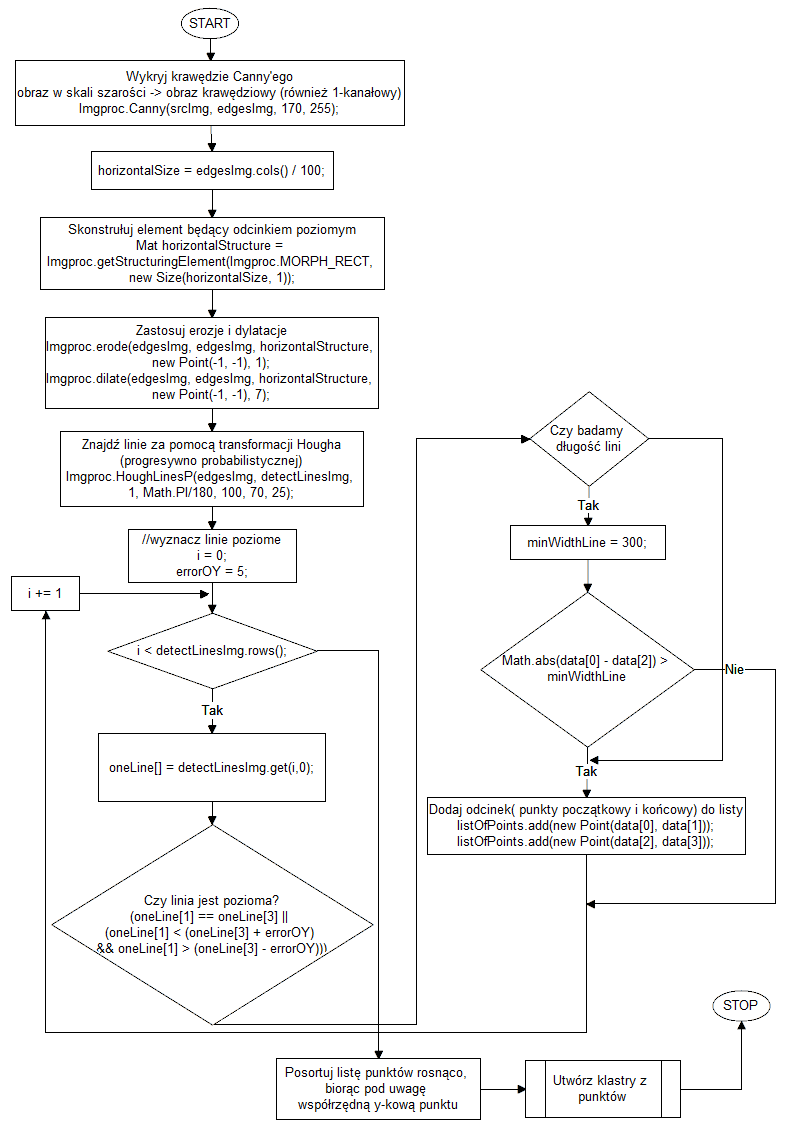
\includegraphics[height=18cm, width=15cm]{image//algorithm//prepareImgToAnalize.png} 
    			    \end{center}
    		    	\caption
        	    		[Algorytm znajdujący linie poziome]  
            			{Algorytm znajdujący linie poziome}  
    		    \end{figure}	
				
    			\begin{figure}[!ht]  
    		        \begin{center}
    		    	    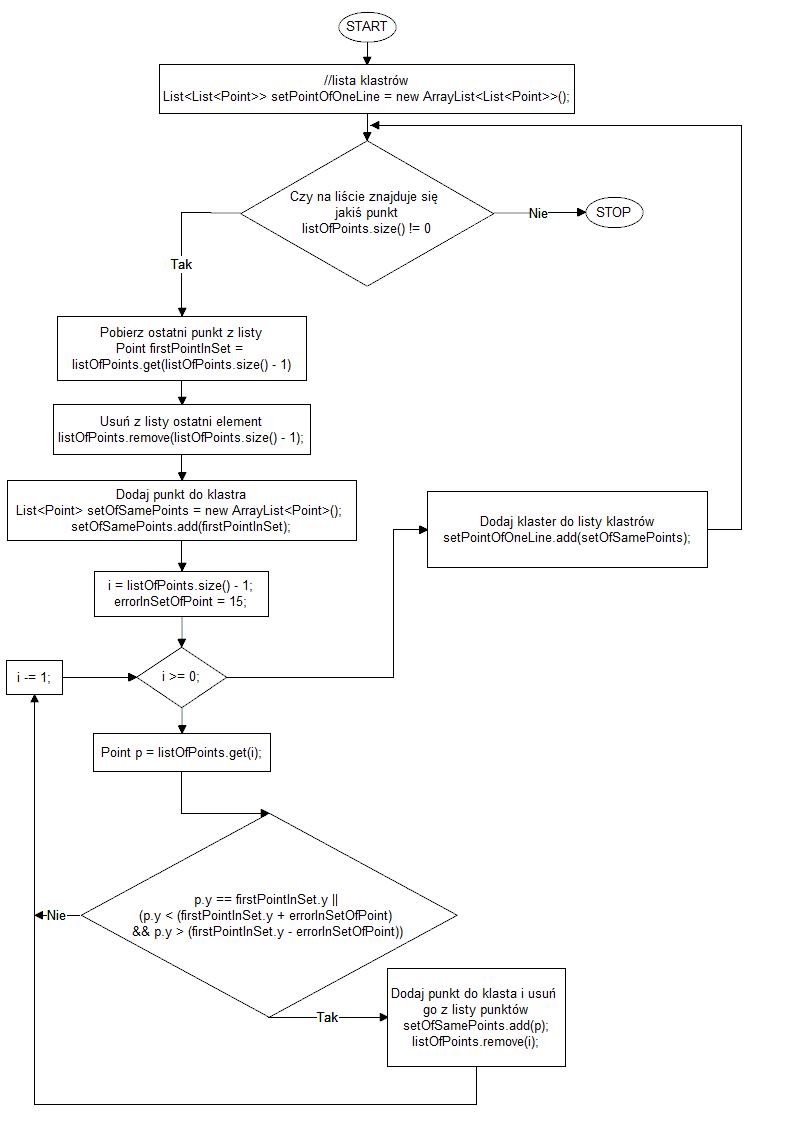
\includegraphics[height=12cm, width=10cm]{image//algorithm//prepareImgToAnalizePred.png} 
    			    \end{center}
        			\caption
        			    [Algorytm budujący listę klastrów]  
            			{Algorytm budujący listę klastrów}  
    		    \end{figure}
		        \newpage
		        Algorytm wykorzystuje zasadnicze przekształcenia morfologiczne udostępnione w bibliotece OpenCv --- dylatacje i erozje, które mają szerokie zastosowanie w zagadnieniu przetwarzania obrazów. \par
		        \textbf{Dylatacja} jest to konwolucja obrazu i jądra, w której wszystkie piksele zostają zastąpione na lokalne maksimumm każdego z pikseli, które obejmuje jądro. Jest to operacja nieliniowa, która powoduje rozrastanie się jasnego obszaru i zazwyczaj powoduje wypełnienie zagłębień przy przyjęciu założenia, że jądro jest jądrem wypukłym i wypełnionym. \par
    		    \textbf{Erozja} jest to operacja przeciwna do operacji dylatacji, a więc piksele zostają zastępione na lokalne minimum, jest to również operacja nieliniowa, która powoduje zmniejszenie się czarnego obszaru oraz usuwa wypukłości, przy tych samych założeniach.
		    
		\subsubsection{Klasa ToStraightenUp}		
		    \paragraph{} Metody tej klasy pomagają zniwelować w pewnym stopniu wp\l yw      ludzki na jakość przetwarzania obrazu. Umożliwiają one wyprostowanie        danego zdjęcia jeśli zostało ono niew\l aściwie, krzywo umieszczone na      skanerze. Klasa ta wykorzystuje również metody klasy PrepareImgToAnalize     dzięki której buduje zbiór linii, z których każda ma taką podobną           wspólrzędna y---kową początku i końca. I na podstawię średniej z różnic     tej wspó\l rzędniej wykrytych linii określany jest kąt o jaki należy        obrócic obraz, tak aby zosta\l on wyprostowany.  
		
		        Algorytm wykorzystuje funkcję zaimplementowaną w bibliotece OpenCv przekształcającą obraz. Jest to funkcja przekształcenia afinicznego:
    		    \begin{center}
    		        \textit{Imgproc.warpAffine(srcImg, dstImg, M, dsize);}.
    		    \end{center}
		    
		        która punkt macierzy źródlowej \textit{srcImg} przekształca do macierzy wynikowej \textit{dstImg} według macierzy określającej jakiego rodzaju jest to przeształcenie \textit{M} mającej dwa wiersze i trzy kolumny według nastepującego wzoru:
                \begin{center}
                    \textit{$dst(x,y) = src( M_{11} x + M_{12} y + M_{13}, M_{21} x + M_{22} y + M_{23}$}.
                \end{center} \par    
                Ponieważ prawa strona równania często nie jest liczbą całkowitą, wartość odpowiedniego punktu macierzy wynikowej oblicza się stosując interpolację. Metoda ta dostarcza również innych wariantów wywołania z kolejnymi argumentami takimi jak: 
            
                \begin{spacing}{1}
                \begin{itemize}
                    \item \textit{flags} --- wybór metody interpolacji( dostępne są następujące typy:\\
                    INTER\_NEAREST --- najbliższego sąsiada,\\ 
                    INTER\_LINEAR --- dwuliniowa,\\
                    INTER\_AREA --- przepróbkowanie obszaru pikseli,\\
                    INTER\_CUBIC --- interpolacja dwusześcianowa,\\
                    INTER\_LANCZOS4 --- interpolacja wykorzystująca metodę Lanczoasa biorąca pod uwagę sąsiednie punkty w obszarze o wymiarach 8x8,\\ 
                    można dołączyć dodatkową opcję przy użyciu operatora lub WRAP\_INVERSE\_MAP --- przekształcenie z \textit{dstImg} do \textit{srcImg}),
                    \item \textit{borderMode} --- metoda użyta do ekstrapolacji pikseli znajdujących sie na zewnątrz obrazu (dostępne są następujące typy:\\
                    BORDER\_CONSTANT --- dodaje piksele o stałej wartości,\\
                    BORDER\_WRAP --- dodaje piksele przez pobranie ich z przeciwnej strony,\\
                    BORDER\_REPLICATE --- dodaje piksele przez skopiowanie ich z krawędzi,\\
                    BORDER\_REFLECT --- dodaje piksele przez lustrzane odbicie,\\
                    BORDER\_REFLECT\_101 --- dodaje piksele przez lustrzane odbicie przy tym nie duplikując pikseli tworzących krawędź,\\
                    BORDER\_DEFAULT --- jest to alias dla BORDER\_REFLECT\_101),
                    \item \textit{borderValue} --- paramentr wżywany w przypadku stałej granicy, wartością domyślną jest zero.  
        		 \end{itemize}
        		 \end{spacing}
		 
        		 \begin{figure}[!ht]  
                    \begin{center}
        	    	    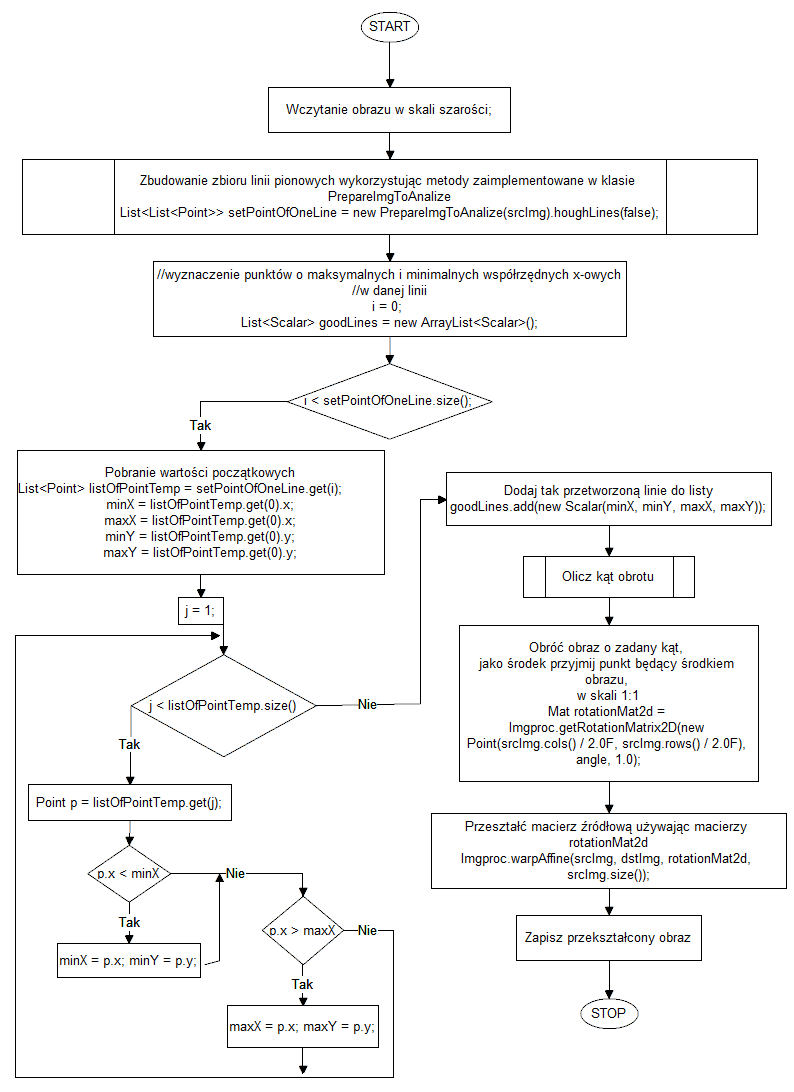
\includegraphics[height=12.5cm, width=10cm]{image//algorithm//toStraightenUp.png} 
    			    \end{center}
        		    \caption
            			[Algorytm obracający obraz tak aby był prosty]  
            			{Algorytm obracający obraz tak aby był prosty}  
        	    \end{figure}
        		 
    		    \begin{figure}[!ht]  
                    \begin{center}
        	    	    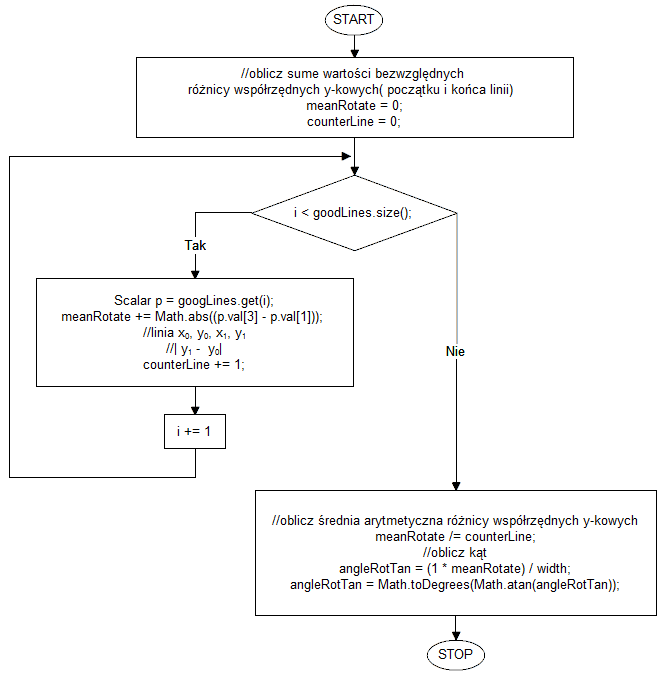
\includegraphics[height=8cm, width=8cm]{image//algorithm//toStraightenUpPred.png} 
    			    \end{center}
        		    \caption
        			    [Algorytm obliczający kąt obrotu]  
        			    {Algorytm obliczający kąt obrotu}  
        	    \end{figure}
		 
        		\begin{figure}[!ht]  
        		    \begin{center}
        			    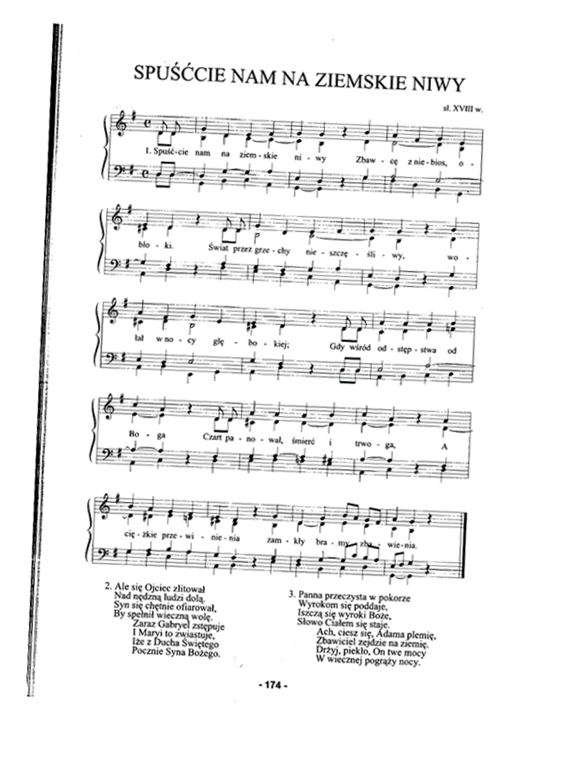
\includegraphics[height=8.25cm, frame]{image//exampleImage//003_a.png} 
        		    \end{center}
        		    \caption
        			    [Obraz przed wyprostowaniem]  
            			{Obraz przed wyprostowaniem}  
        	    \end{figure}
        			
                \begin{figure}[!ht]  
        		    \begin{center}
        			    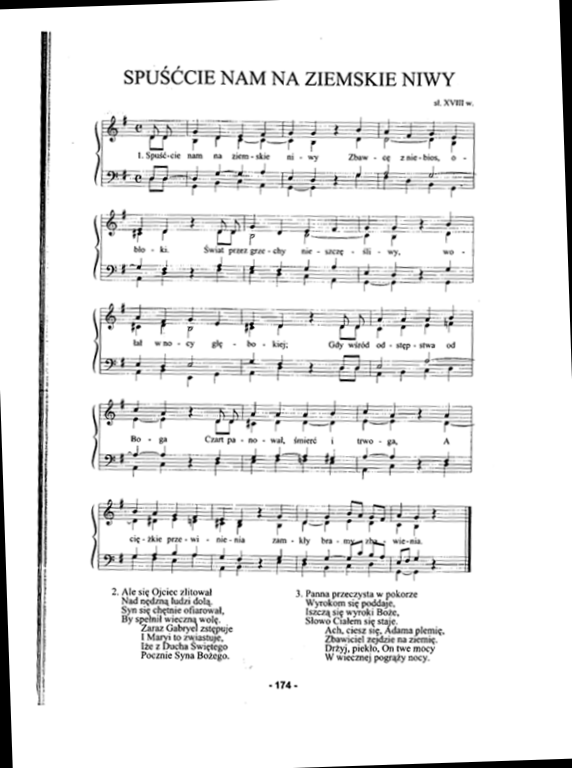
\includegraphics[height=8.25cm, frame] {image//exampleImage//003_b.png} 
        		    \end{center}
        			\caption
            			[Obraz po wyprostowaniu]  
            			{Obraz po wyprostowaniu}  
        	    \end{figure} 
		
		        \newpage 
		 
	    \subsubsection{Klasa MajorProcessing}
		    \paragraph{} Metody tej klasy również używają algorytmów zaimplementowanych     w klasie PrepareimgToAnalize. Wykryte linie transformatą Hougha zostają     pogrupowane w zbiory tworzące pięciolinie. Odpowiednio w zależności od      budowy śpiewnika z jedna pięciolinią( klucz wiolinowy) z tekstem            umieszczonym pod nią lub zdwiema pięcioliniami oraz tekstem umieszczonym     pomiędzy nimi. Następnie wykryte pięcioline zostają zamarkowane             utwarzając bounding boxy i wraz z tekstem znajdującym sie pod lub między     nimi wycięte z obrazu i zapisane do osobnych plików czy macierzy            przechowujących obrazy, a więc przygotowane do dalszego przetworzenia i     ostatecznego uzyskania z nich tekstu.
		
			\begin{figure}[!ht]  
			    \begin{center}
				    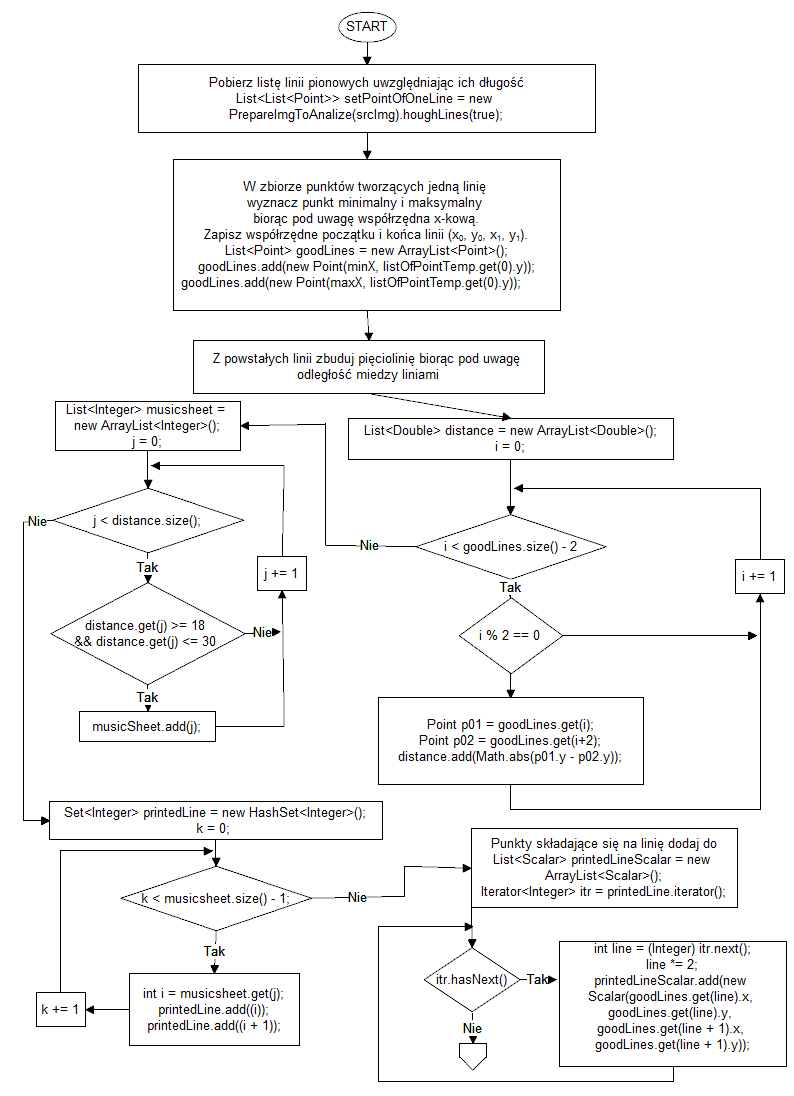
\includegraphics[height=17cm]{image//algorithm//majorProcesing_01.png} 
			    \end{center}
			    \caption
    			    [Główny algorytm budujący bounding boxy cz. 1]  
    			    {Główny algorytm budujący bounding boxy cz. 1}  
		    \end{figure}
			
			\newpage
			
	        \begin{figure}[!ht]  
			    \begin{center}
				    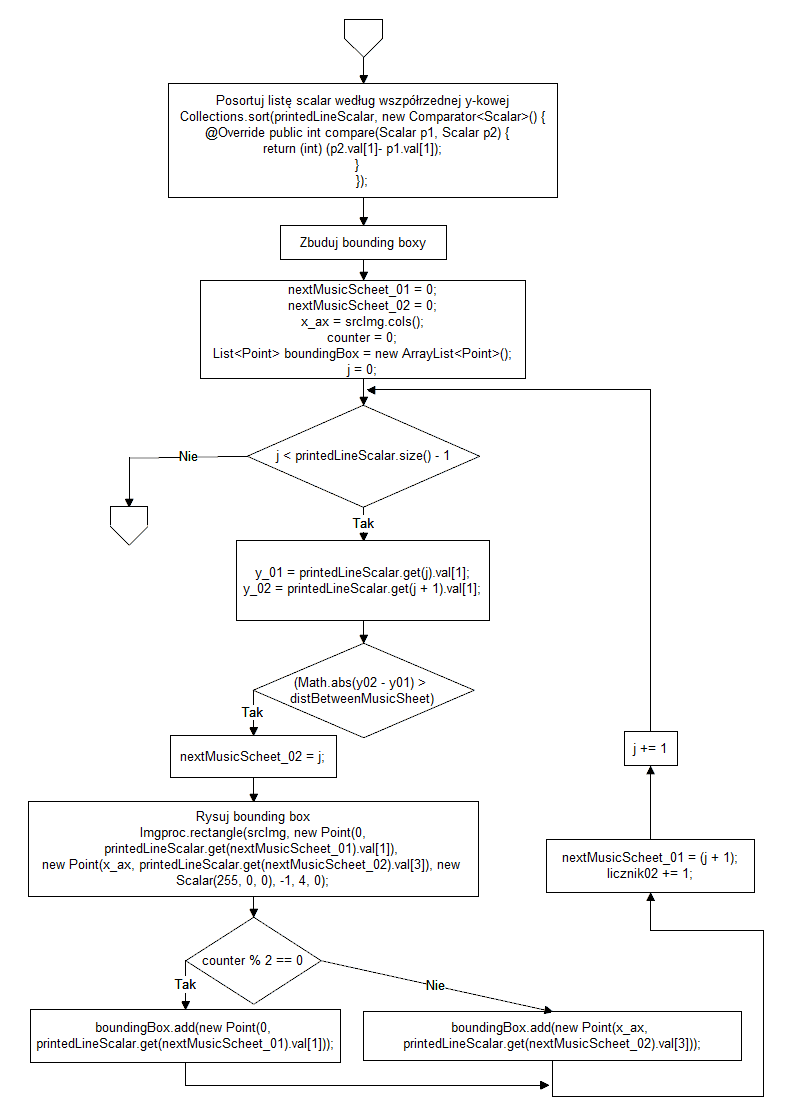
\includegraphics[height=12cm] {image//algorithm//majorProcesing_02.png} 
			    \end{center}
			    \caption
    			    [Główny algorytm budujący bounding boxy cz. 2]  
    			    {Główny algorytm budujący bounding boxy cz. 2}  
		    \end{figure} 
		
		    \begin{figure}[!ht]  
			    \begin{center}
				    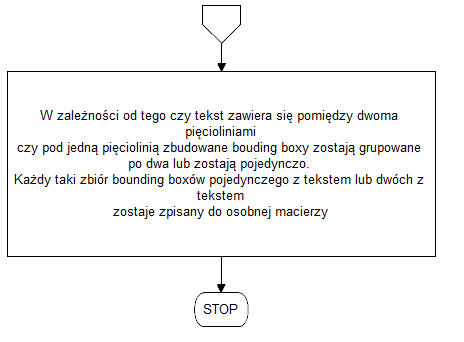
\includegraphics[height=8cm] {image//algorithm//majorProcesing_03.png} 
			    \end{center}
			    \caption
    			    [Główny algorytm budujący bounding boxy cz. 3]
    			    {Główny algorytm budujący bounding boxy cz. 3}  
		    \end{figure} 
		
    		\begin{figure}[!ht]  
			    \begin{center}
				    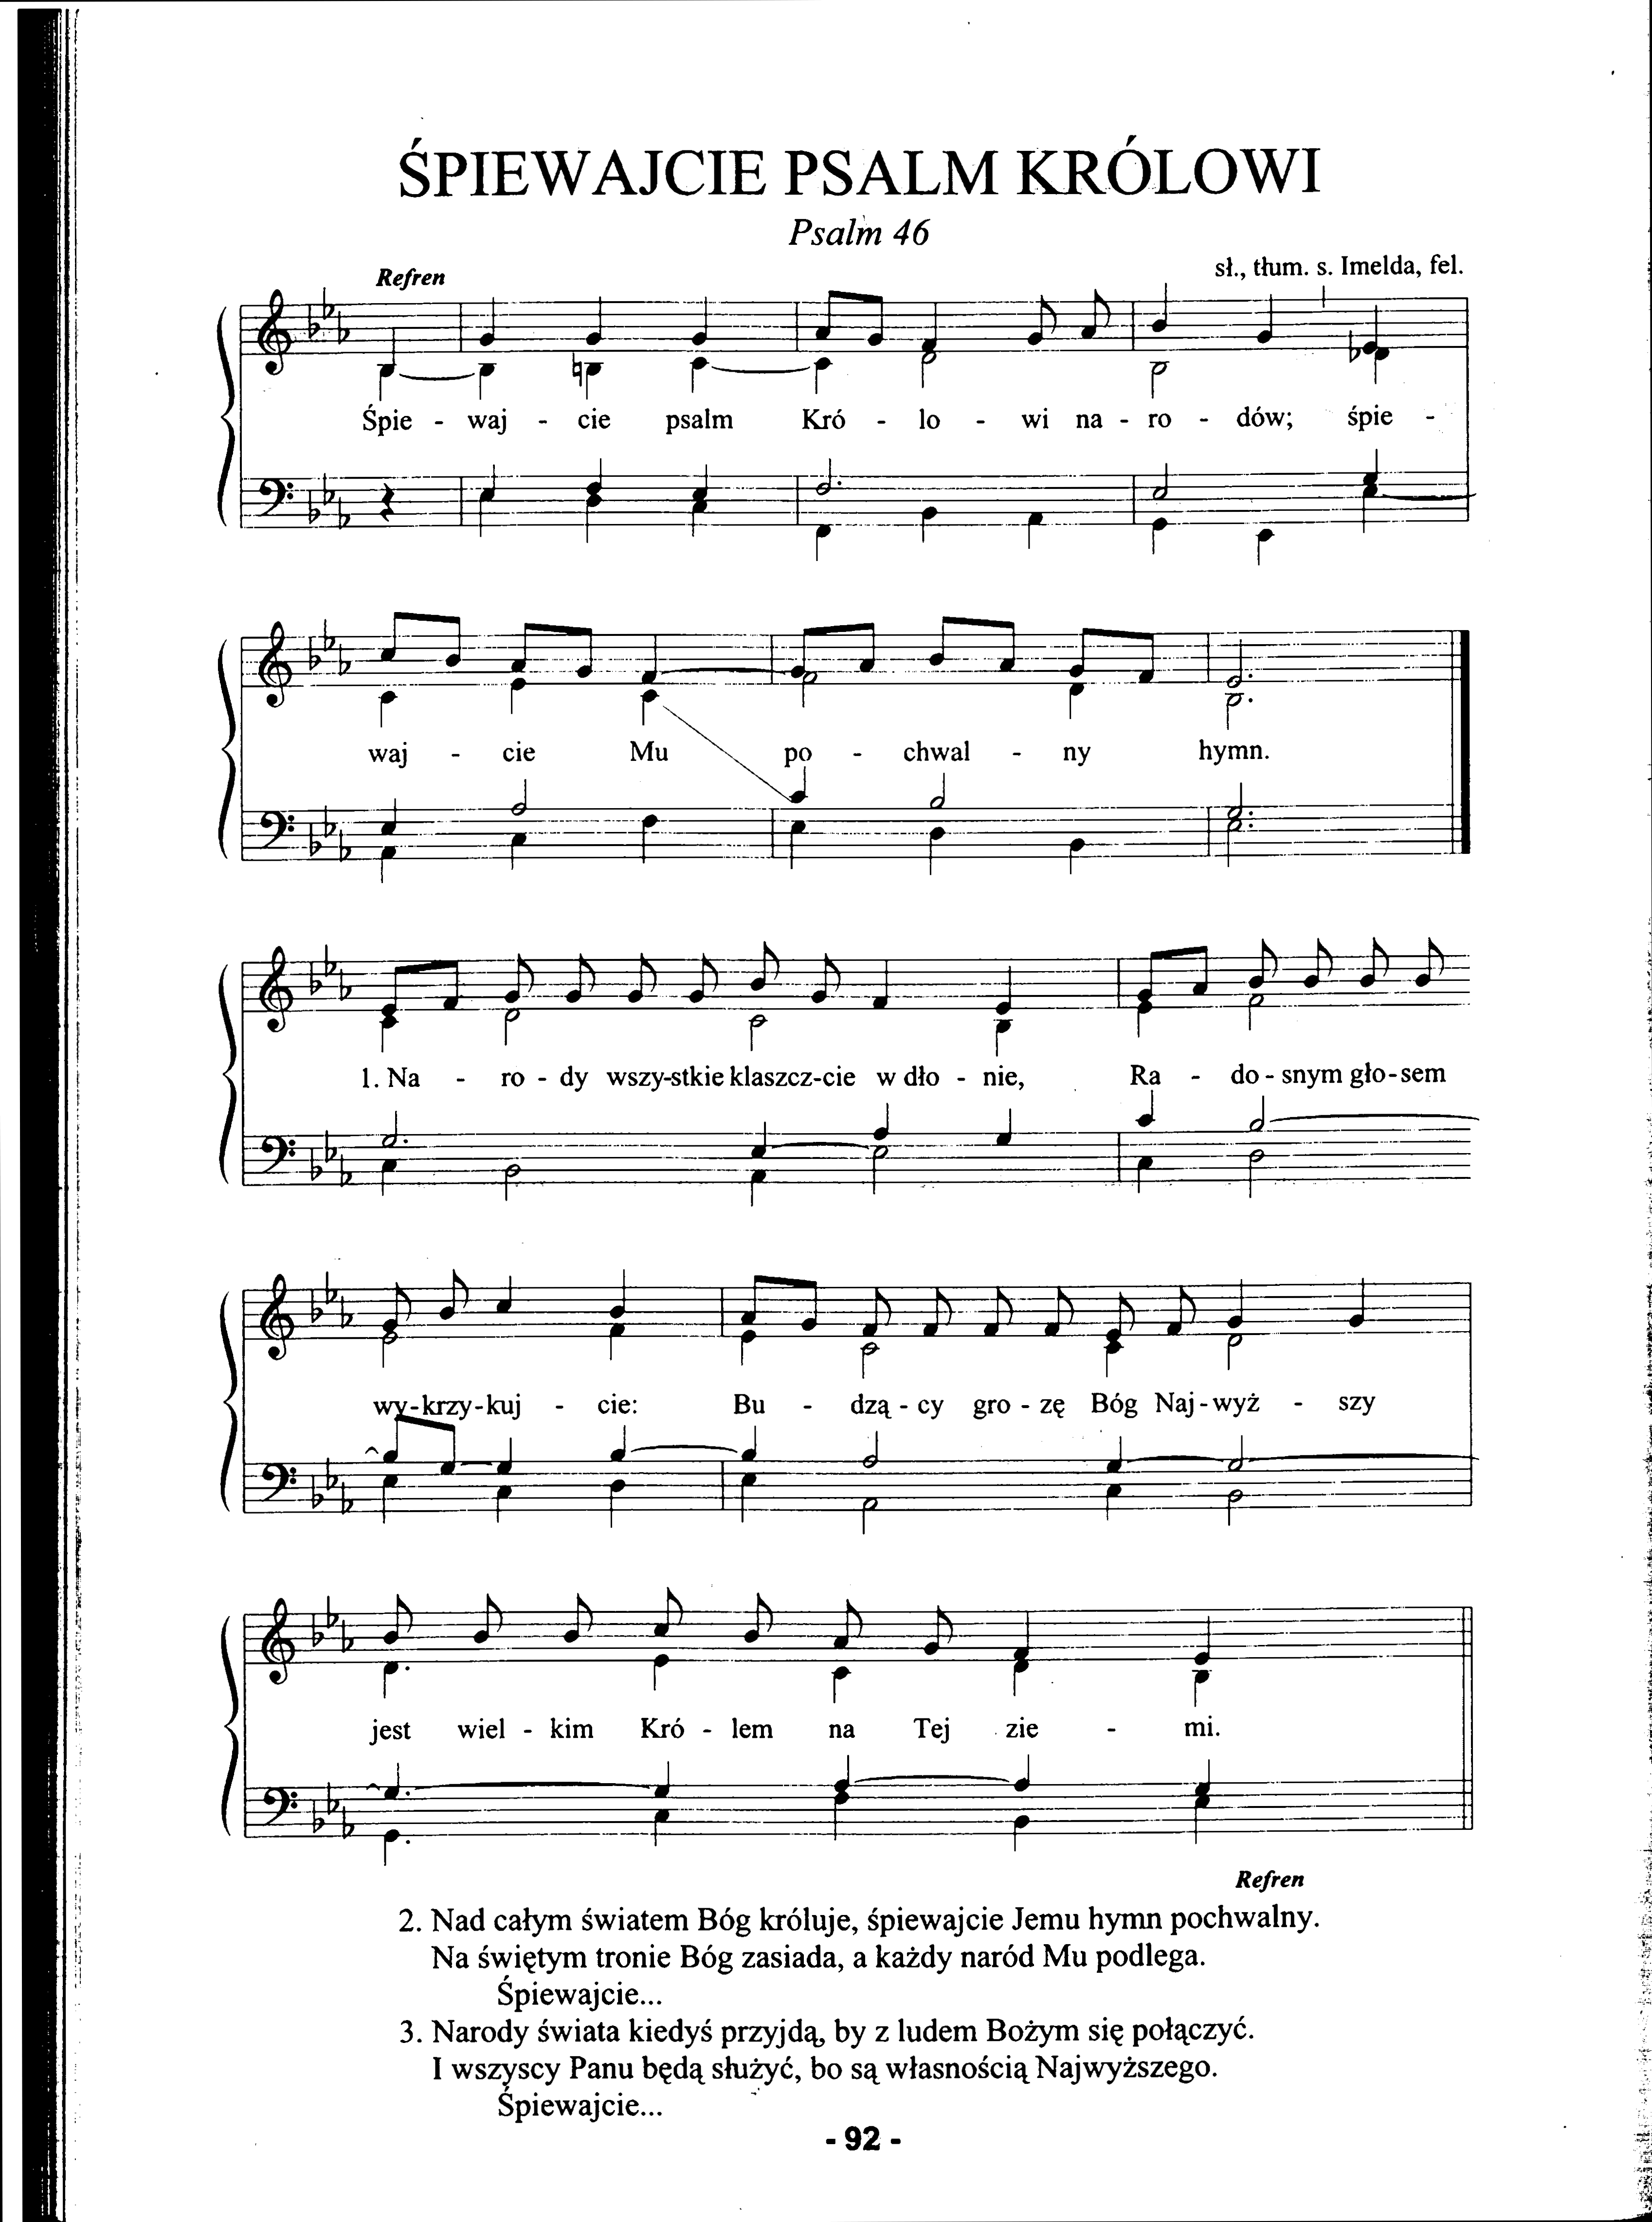
\includegraphics[height=8.25cm, frame] {image//exampleImage//004_a.png} 
			    \end{center}
			    \caption
    			    [Obraz przed wykryciem pięciolinii]  
    			    {Obraz przed wykryciem pięciolinii}  
		    \end{figure} 
		
		    \begin{figure}[!ht]  
			    \begin{center}
				    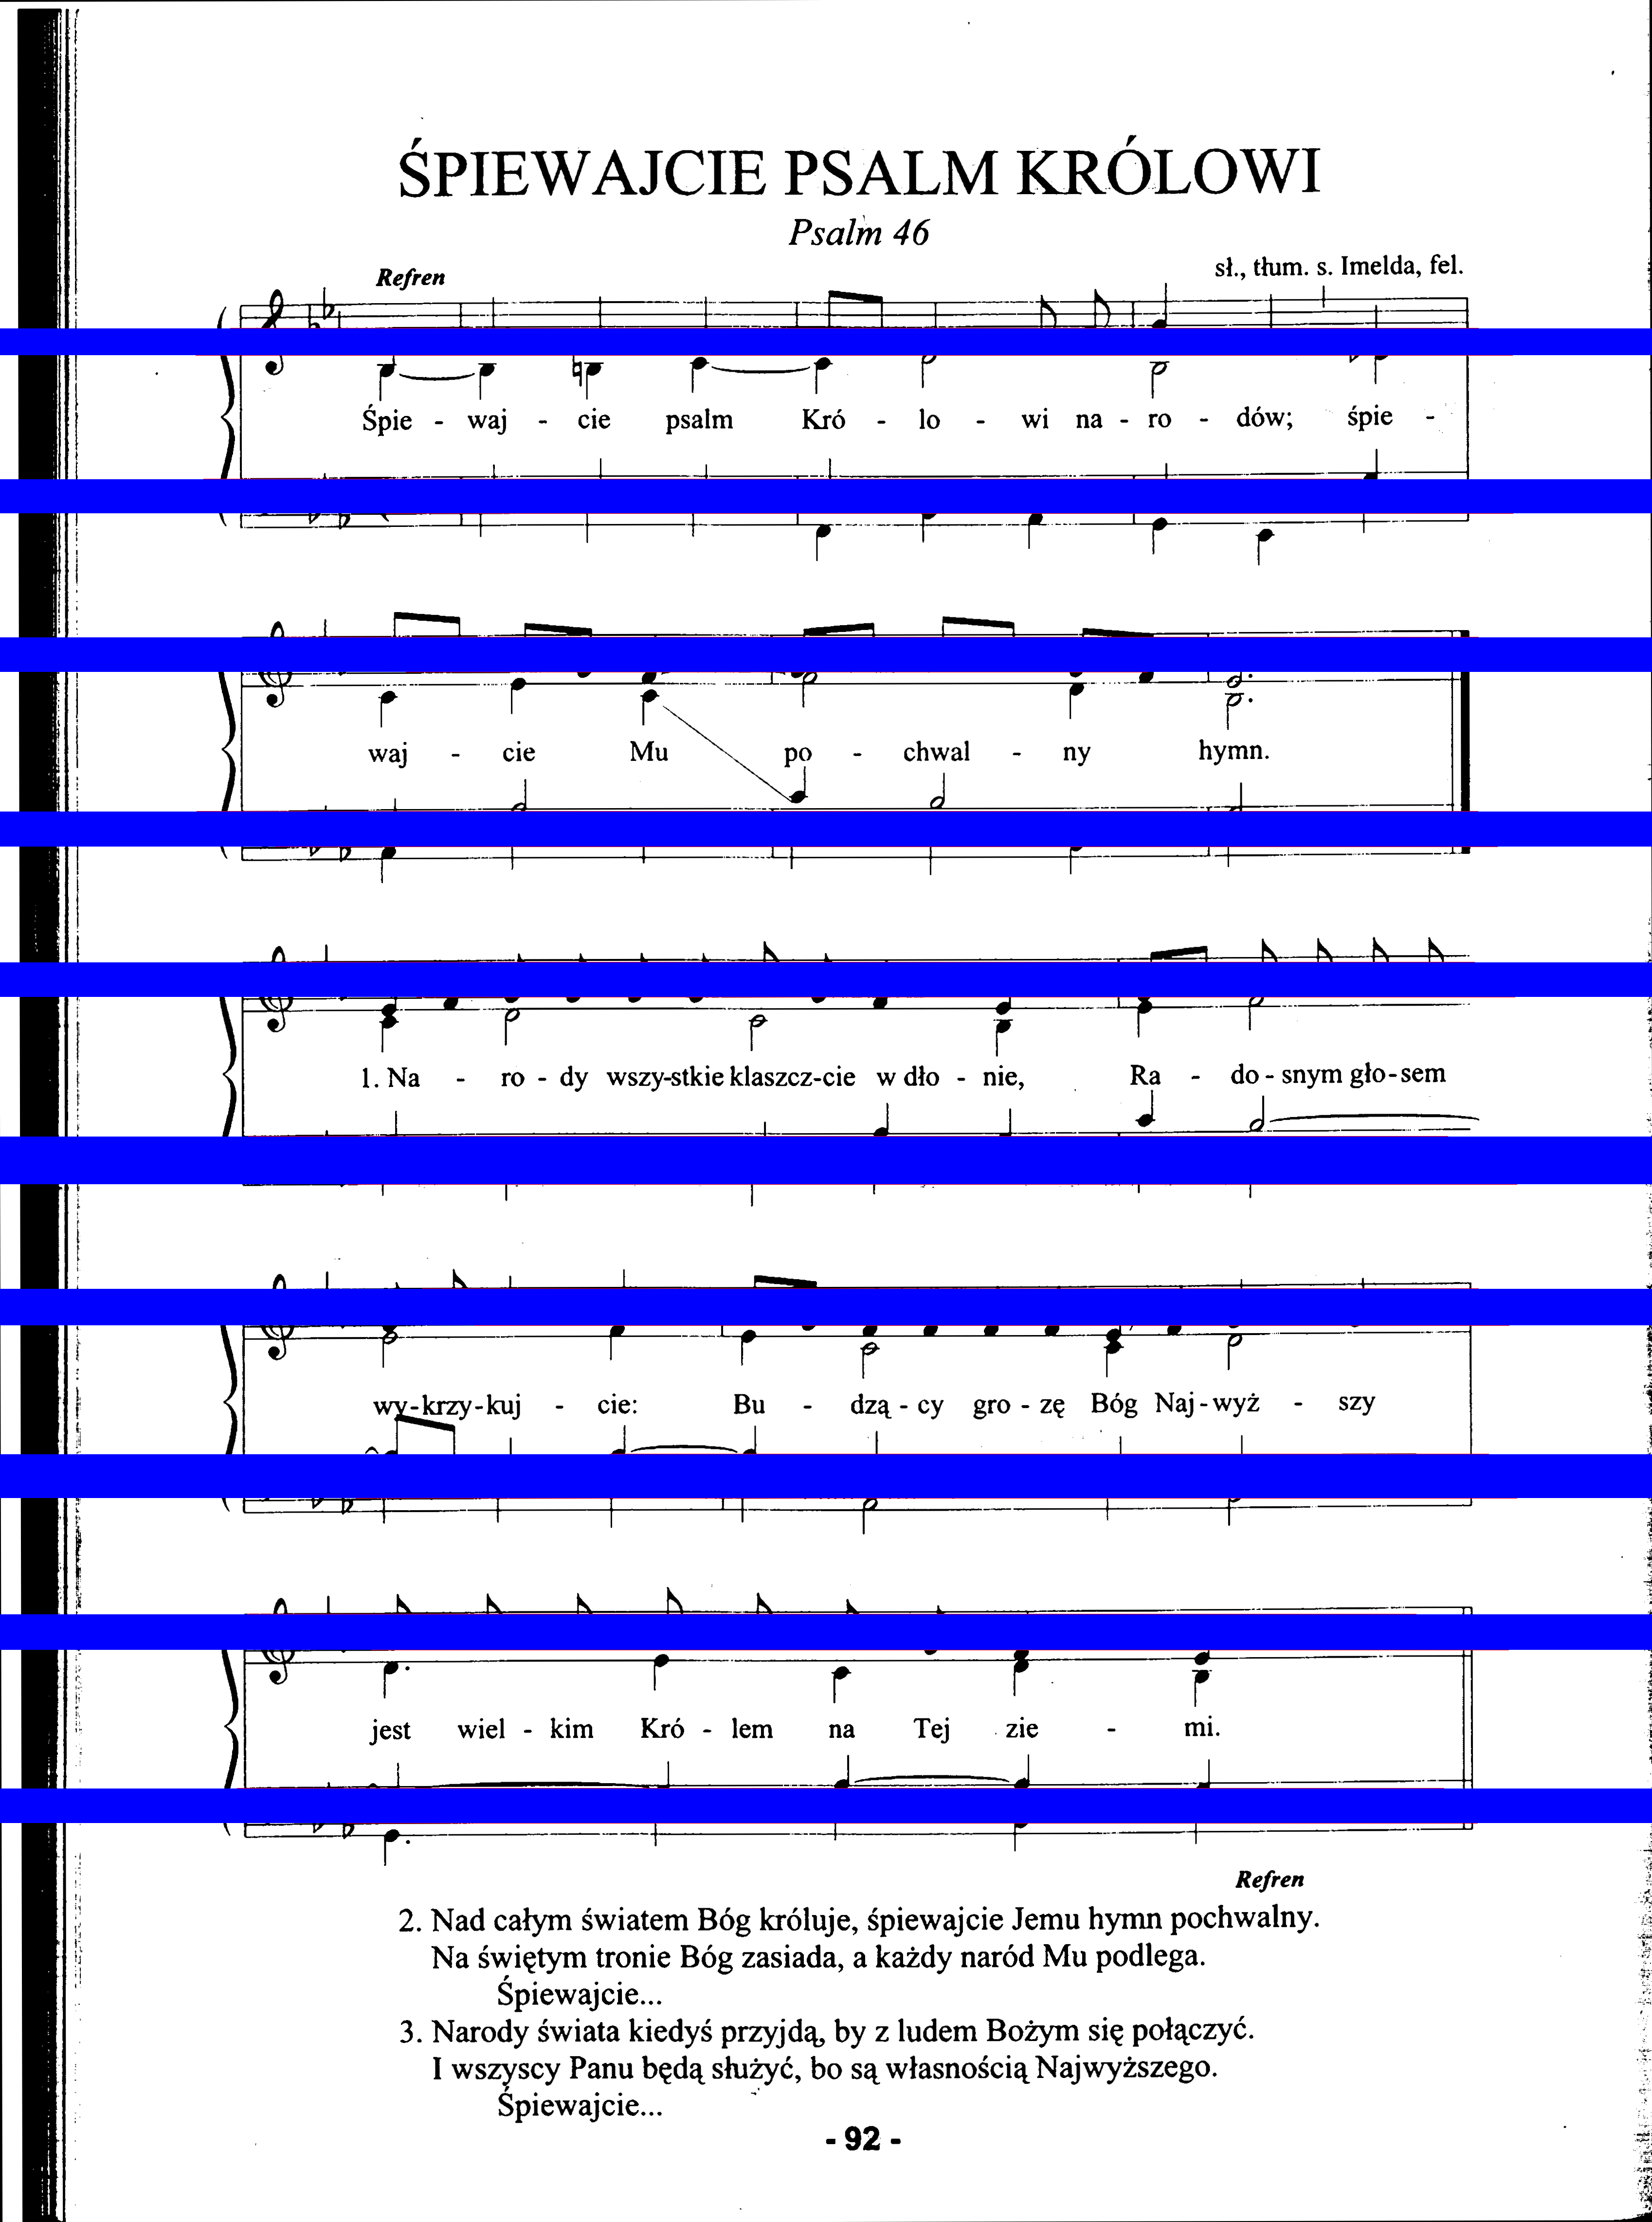
\includegraphics[height=8.25cm, frame] {image//exampleImage//004_b.png} 
			    \end{center}
			    \caption
    			    [Obraz po wykryciu pięciolinii]  
    			    {Obraz po wykryciu pięciolinii}  
		    \end{figure} 
		
		\subsubsection{Klasa MusicSheetClassifier}  
	        \paragraph{} Klasa zawiera model konwolucyjnej sieci neuronowej który           zostaje ''nauczony'' klasyfikacji obrazów wejściowych na zawierające        tekst lub  pięciolinię, na podstawie wcześniej przygotowanych zdjęć         treningowych( jednokanałowych, o roazmiarzach 600px x 15px).
		
    		\begin{figure}[!ht]  
	    	    \begin{center}
	    		    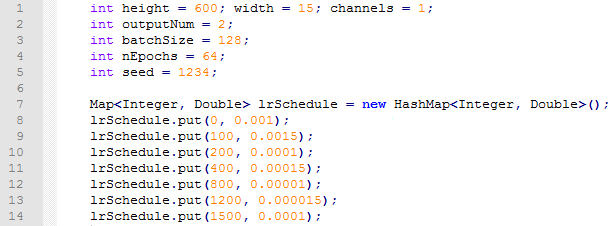
\includegraphics[width=15cm, frame] {image//practicalPart//cnnConf_03.png} 
	    	    \end{center}
		    \end{figure}
                
	        \begin{figure}[!ht]  
    		    \begin{center}
    			    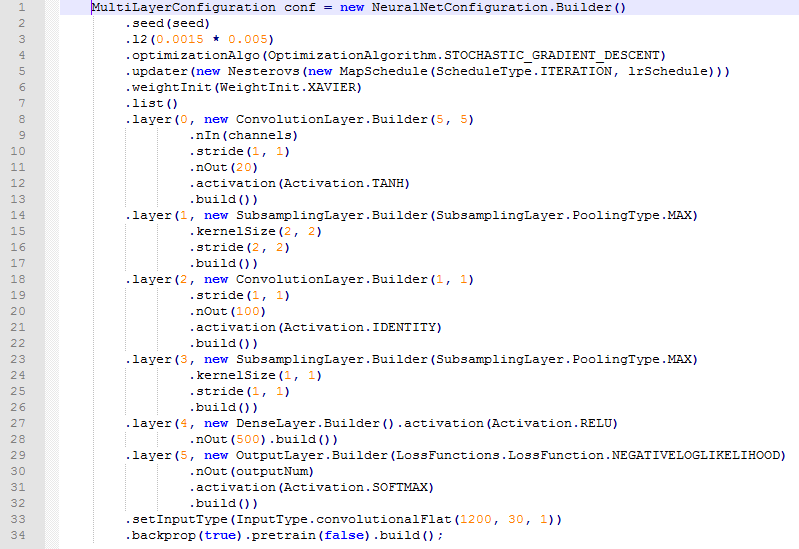
\includegraphics[width=15cm, frame] {image//practicalPart//cnnConf_04.png} 
    		    \end{center}
		    \end{figure}  
		
            \begin{spacing}{1.5}
		    \begin{center}
                \begin{tabular}{c c c }
                    \# of classes: & liczba klas & 2 \\
                    Accuracy:  & dokładność &0,9806  \\ 
                    Precision:  & precyzja & 0,9768 \\  
                    Recall: & wycofanie & 0,9808      \\
                    F1 Score: & rezultat f1 & 0,9851
                \end{tabular}
            \end{center}
		    \end{spacing}
		 Konfiguracja sieci neuronowej: 
		    \begin{spacing}{1}
            \begin{itemize}
                \item lrSchedule - współczynnik, krok( x) z jakim uczy się siec w n-tej iteracji \textbackslash\textbackslash  \vspace{2cm} lrSchedule.put(n, x);
                \item seed - losowa liczba, używana na potrzeby powtarzalności;
                \item l2 - reguzlaryzacja l2;
                \item optimizationAlgo - algorytm optymalizacji dotyczy działania parametrów określonych w updater. Stochastic gradient descent wykonuje optymalizację, której celem jest znalezienie maksimum w danym przedziale. Optymalizacja obejmuje obliczenie wartości błędu i zmianie wag w celu osiągnięcia minimalnego błędu;
                \item updater - określa współczynniki uczenia się sieci;
                \item weightInit - inicjalizacja wag sieci neuronowej. Xavier jest zazwyczaj właściwym parametrem, aby zainicjowane wagi nie były zbyt duże ani zbyt niskie;
            \end{itemize}
            \end{spacing}
            
            Dalsza konfiguracja sieci sklada się z warstw wykonujących konwolucję ConvolutionLayer i warstw wykonujących pooling SubsamplingLayer. 
            
            \begin{spacing}{1}
            \begin{itemize}
                \item ConvolutionLayer.Builder(x, y) - określa wiekość jądra warstwy konwolucyjnej;
                \item nIn(channels) - określa liczbę kanałów obrazu wejściowego;
                \item stride(n, m) - mówi nam o kroku z jakim jądro przechodzi przez obraz wejściowy;
                \item nOut(k) - określa liczbę filtrów przez które przechodzi obraz; 
                \item activation() - funkcja aktywacji;
                \item SubsamplingLayer.Builder(SubsamplingLayer.PoolingType.MAX) - warstwa odpowiadająca za pooling określonego rodzaju; 
                \item kernelSize(x, y) - rozmiar jadra;
                \item DenseLayer.Builder() - warstwa przetwarzająca wszzystkie wyniki z warstwy poprzedniej; 
                \item nOut(500) - okresla liczbe wyjsc;
                \item OutputLayer.Builder(LossFunctions.LossFunction.NEGATIVELOGLIKELIHOOD) - wyjściowa warstwa ukryta z okreslona funkcja straty.
            \end{itemize}
		\end{spacing}
		
		\subsubsection{Klasa DetextText} 		
			\paragraph{} Algorytmy zaimplementowane w tej klasie umożliwiają w              dotychczas przygotowanych obrazach, maksymalnie rozszerzyć obszar           powsta\l ych bounding boxów na podstawie odchylenia standardowego, co       umożliwia praktycznie ca\l kowite usunięcie znaków muzycznych( nut i        pięciolinii). Obszar w którym prawdopodobnie znajduje się tekst zostaje     wycięty i jest obrazem wejściowym dla konwolucyjnej sieci neuronowej        która podejmuje decyzje czy jest on linią tekstu czy nut. Jeśli sieć        zwróci wartość pozytywną( obraz jest tekstem; prawdopodobieństwo wieksze     niż 0.9), zostaje on wycięty i poddany dalszej obróce, zaś jeśli sieć       zwróci wartość negatywną( obraz nie jest tekstem; prawdopodobieństwo        mniejsze lub równe 0.9) dlaszemu przetwarzaniu zostaje poddany cały         obraz.  

			    \begin{figure}[!ht]  
			        \begin{center}
				        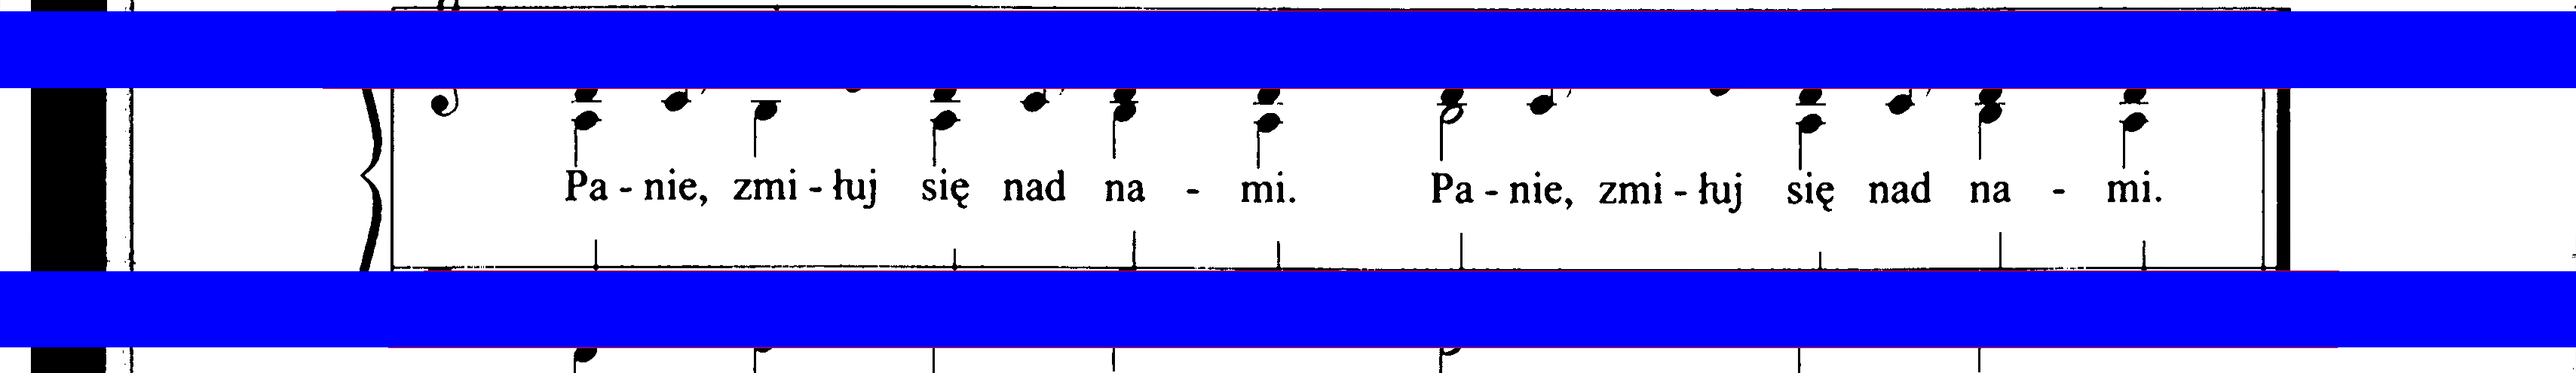
\includegraphics[width=15cm, frame] {image//exampleImage//005_a.png} 
			        \end{center}
			        \caption
    			        [Obraz przed rozszerzeniem bounding boxów]  
    			        {Obraz przed rozszerzeniem bounding boxów}  
		        \end{figure} 
		
		        \begin{figure}[!ht]  
			        \begin{center}
				        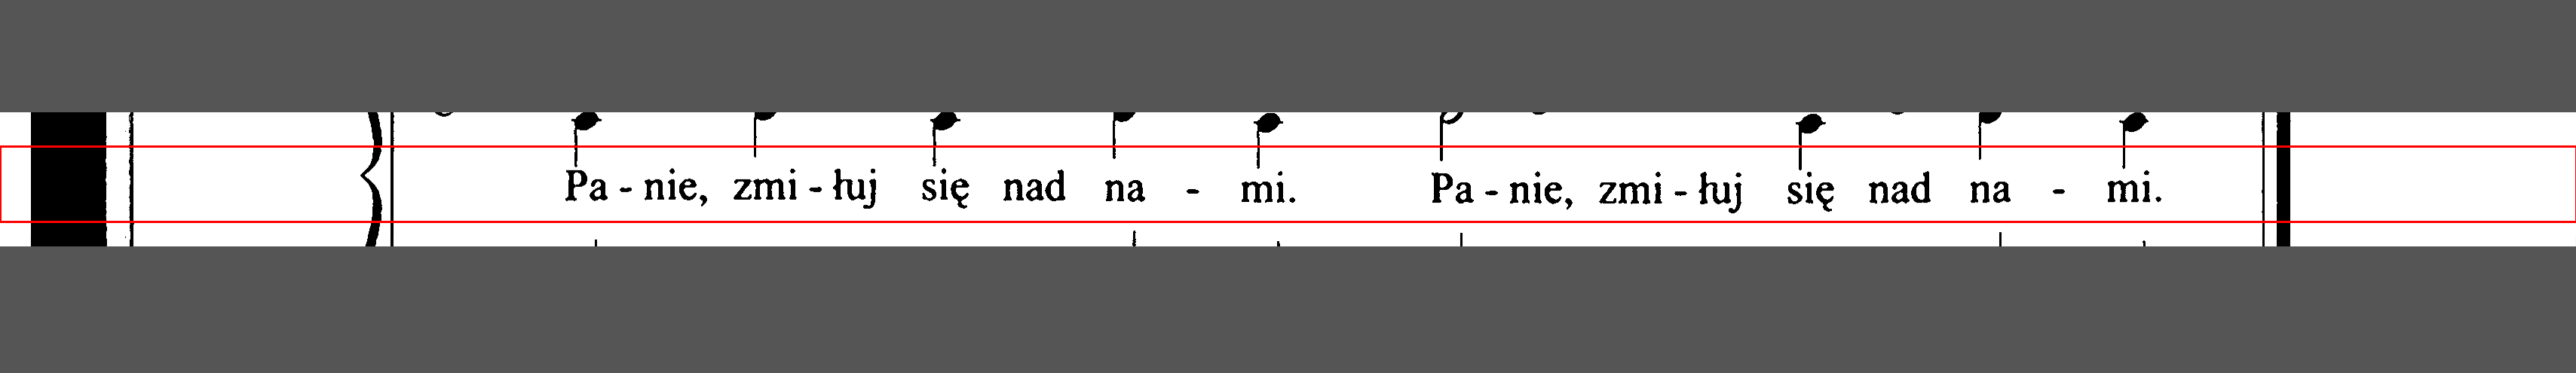
\includegraphics[width=15cm, frame] {image//exampleImage//005_b.png} 
			        \end{center}
			        \caption
    			        [Obraz po rozszerzeniu bounding boxów i zamarkowaniu miejsca gdzie znajduje się tekst]  
    			        {Obraz po rozszerzeniu bounding boxów i zamarkowaniu miejsca gdzie znajduje się tekst}  
		        \end{figure} 
		    
		        \begin{figure}[!ht]  
			        \begin{center}
				        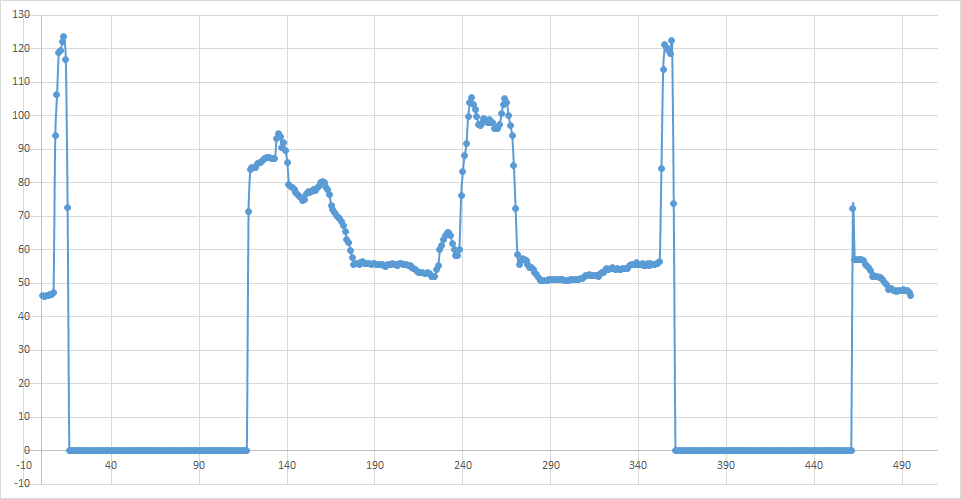
\includegraphics[width=12cm, frame] {image//practicalPart//stdDevDetectText.png} 
			        \end{center}
			        \caption
        			    [Wykres odchylenia standardowego poszczególnych linii]  
        			    {Wykres odchylenia standardowego poszczególnych linii}  
		        \end{figure}
		    
		    Na podstawie wykresu możemy zauważyć ze tekst znajduje się pomiędzy dwoma większymi obszarami o wartościach zerowych, dokladniej pomiędzy liniami od około 240 do około 270, odchylenie standardowe wierszy zawierających tekst waha się w zakresie od około 95 do około 105. Obszar pomiędzy tekstem a zamarkowanymi pięcioliniami ma niezbyt duże odchylenie standardowe ponieważ mogą się w tych liniach znajdować nuty dodane, ogonki nut jednak nie będzie ich nigdy zbyt wiele i rozrzut w tych liniach nie będzie większy od rozrzutu w liniach w których znajdują się litery.

        \subsubsection{DetectLetter}
            \paragraph{} Algorytmy tej kalsy wykrywają krawędzie w obrazie wejściowym,     następnie grupują je w zbiory o taki samych współrzędnych x-owych, dzięki    czemu jedna grupa konturów stanowi jeden znak (literę, znak                 interpunkcyjny, etc.), grupy są sortowane rosnąco według współrzednych      x-owych. Z każdego zbioru konturów zostają wyznaczone skrajne współrzędne    $ max_{x} , min_{x}, max_{y}, min_{y} $. Na podstawie tych wartości z       obrazu wejsciowego zostaje wycięty kontur zawierający się w tym             prostokącie. Tak wyciętemu obrazowi zostaje nadana jednoznaczna nazwa       według jego indeksu w zbiorze posortowanym. 
    
            \begin{figure}[h!]
                \centering
                \begin{subfigure}[b]{2cm}
                    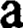
\includegraphics[width=1.5cm, height=1.5cm, frame]{image//exampleImage//letter_01.png}
                    \caption{}
                \end{subfigure}
                \begin{subfigure}[b]{2cm}
                    
\includegraphics[width=1.5cm, height=1.5cm, frame]{image//exampleImage//letter_02.png}
                \caption{}
                \end{subfigure}
                \newline
                \begin{subfigure}[b]{2cm}
                    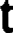
\includegraphics[width=1cm, height=2cm, frame]{image//exampleImage//letter_03.png}
                    \caption{}
                \end{subfigure}
                \begin{subfigure}[b]{2cm}
                    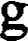
\includegraphics[width=1cm, height=2cm, frame]{image//exampleImage//letter_04.png}
                    \caption{}
                \end{subfigure}
                \caption
                [Przykladowe wycięte litery]
                {Przykladowe wycięte litery}
                %\label{}
            \end{figure}

        \subsubsection{LetterClassifier}
            \paragraph{} Klasa zawiera model konwolucyjnej sieci neuronowej który           zostaje ''nauczony'' rozpoznawania liter abecadła, w tym polskich znaków     diakrytycznych, majuskuł i minuskuł( łącznie 64 znaki, klasy), na           podstawie wcześniej przygotowanych zdjęć treningowych( jednokanałowych,     o roazmiarzach 50px x 25px), Konfiguracja sieci rózni się od poprzedniej     jedynie kilkoma parametrami i dodatkowymi dwoma warstwami:                  ConvolutionLayer.Builder(x, y) i 
                SubsamplingLayer.Builder(SubsamplingLayer.PoolingType.MAX).
	       
	            \begin{figure}[!ht]  
	    	        \begin{center}
	    		        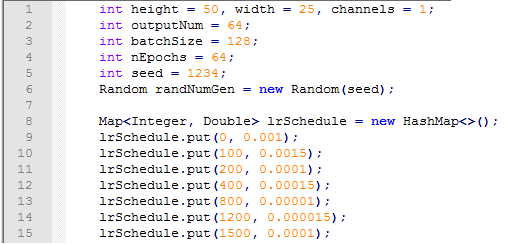
\includegraphics[width=15cm, frame] {image//practicalPart//cnnConf_01.png} 
	    	        \end{center}
		        \end{figure}
            
	            \begin{figure}[!ht]  
    		        \begin{center}
    			        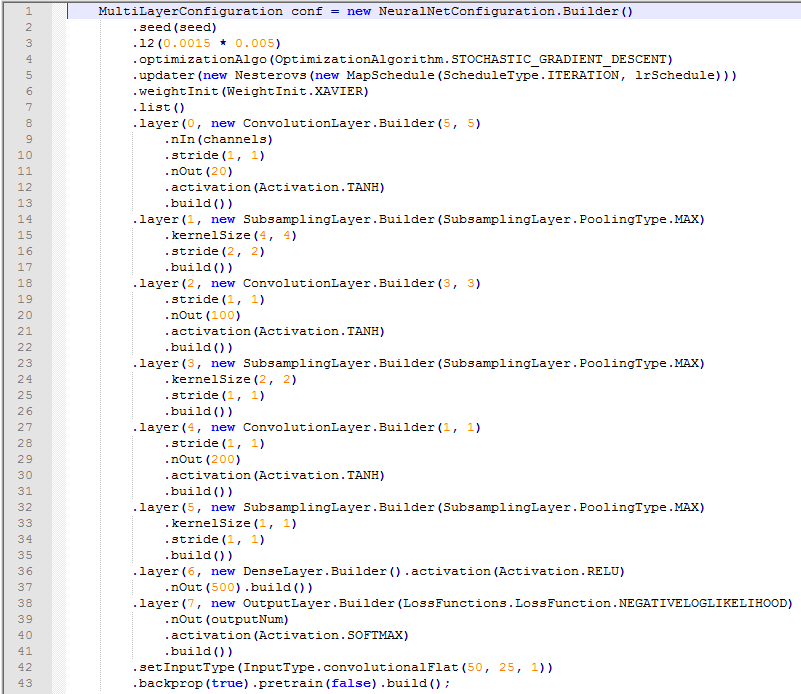
\includegraphics[width=15cm, frame] {image//practicalPart//cnnConf_02.png} 
    		        \end{center}
		        \end{figure}            
            Trening sieci neuronowej daje dość zadowalające wyniki 
    
            \begin{spacing}{1.5}
                \begin{center}
                \begin{tabular}{ c c c  }
                    \# of classes: &  liczb klas & 64 \\
                    Accuracy:  & dokładność & 0,7387  \\ 
                    Precision:  & precyzja & 0,7098 \\  
                    Recall: & wycofanie & 0,5776      \\
                    F1 Score: & rezultat f1 & 0,6347
                \end{tabular}
                \end{center}
            \end{spacing}
            
            Sieć bardzo dobrze rozpoznaje( zwraca wysokie prawdopodobieństwo > 0.9) pojedyncze litery podobne do tych ze zbioru na których się uczy. Podczas pracy ze zbiorem danych ze spiewników nie zawsze algorytm rozpoznawania konturów pojedynczych liter zwraca zadowalające wyniki( same pojedyncze litery ) często gdy kontury liter zachodzą na siebie zwraca kilka liter w jednym obrazie lub dodatkowych znaków co uniemożliwia poprawne rozpoznanie przez sieć. 

            \begin{figure}[h!]
                \centering
                \begin{subfigure}[b]{2cm}
                    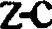
\includegraphics[frame]{image//practicalPart//w_letter_01.png}
                \caption{}
                \end{subfigure}
                \begin{subfigure}[b]{2cm}
                    
\includegraphics[frame]{image//practicalPart//w_letter_02.png}
                \caption{}
                \end{subfigure}
              \newline
                \begin{subfigure}[b]{2cm}
                    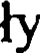
\includegraphics[frame]{image//practicalPart//w_letter_03.png}
                \caption{}
                \end{subfigure}
                \begin{subfigure}[b]{2cm}
                    
\includegraphics[frame]{image//practicalPart//w_letter_04.png}
                    \caption{}
                \end{subfigure}
                \caption
                    [Przykladowe litery wycięte niepoprawnie]
                    {Przykladowe litery wycięte niepoprawnie}
                %\label{}
            \end{figure}

        \subsubsection{ReadLetterClassifier}
	        \paragraph{} ReadLetterClassifier algorytmy tej kalsy odczytują przygotowany     przez klasę DetectLetter obraz zawierający znak, następnie obraz ten        zostaję analizowany przez system OCR Tesseract oraz konwolucyjną sieć       neuronową. Wybranie najbardziej prawdopodobnej litery odbywa się przez      porównanie wyniku zwróconego przez system OCR i trzech największych         prawdopodobieństw zwróconych przez sieć. Tak odczytany cały wykryty         tekst znajdujący się na stronie zostaje zapisany do pliku tekstowego.
	        
	   \newpage  
	   \section{Podsumowanie}
	   \par W niniejszej pracy dyplomowej zostały zrealizowane główne jej założenia. Opracowane algorytmy umożliwiają pozyskanie tekstu ze stron zawierających znaki muzyczne. Identyfikacją liter składających się na poszczególne wyrazy może zostać jescze polepszona, przede wszystkim przez wykorzystnie dokładniejszych algorytmów wycinających poszczególne litery, powiększenie zbioru liter( majuskuł, minuskuł) i linii( tekstu, pięciolinii) na których uczyą się sieci neuronowe. Dzięki zastosowanią sztucznej inteligencji opracowane algorytmy są bardziej uniwersalne i umożliwią pracę ze znacząca liczbą powszechnie wykorzystywanych spiewników wpisujących się w następujące dwa schematy [pięciolinia tekst pieciolinia], [pięciolinia tekst]. Dzięki wytworzeniu oprogramowania zgodznie z zasadami programowania zoriętowanego obiektowo, z łatwością możemy do powyższych dwóch struktur dodawać kolejne w róznych konfiguracjach na przykład [pięciolinia tekst pieciolinia pięciolinia]. 
	   
	   
	   
	   %Jednym z celów pracy, które niestety nie udalo się zrealizować było budowa graficznego interfejsu użytkownia, jednak wybrana technologia i architektura systemu umożliwiają dość proste przejście z aplikacji konsolwej do aplikacji posiadającej przejrzysty i przyjazny dla użytkownika interfejs. 
	   \par 
	   
	   
	   
	   W rozpoznanej treści możemy odnaleźć poszczególne sylaby i wyrazy oraz dzięki ludzkiej percepcji poprawnie odczytać dny wyraz, jednak 
	   
	   \newpage
	   \section{Bibliografia}
	   \subsubsection*{Źródła książkowe:}
	   \begin{itemize}
	        \item Rączkowski F., Śpiewajmy Bogu, Płock, Hejnał, 2012;
	        \item Siedlecki J., Śpiewnik kościelny, Wyd. XL (poprawione), Kraków,
	        Instytut Teologiczny Księży Misjonarzy, 2011;
	        \item Kaehler A., Bradski G., OpenCV 3. Komputerowe rozpoznawanie obrazu w C++ przy użyciu biblioteki OpenCV, Gliwice, Helion, 2017;
	        \item Shanmugamani R., Deep Learning for Computer Vision, Birmingham, Packt Publishing, 2018
	   \end{itemize}
	   
	   
	   \subsubsection*{Źródła internetowe:}
	   Data dostępu 2018.07.15
	   \begin{itemize}
            \item \href{https://opencv.org}{\url{https://opencv.org}}
            \item \href{https://docs.opencv.org//3.1.0//index.html}{\url{https://docs.opencv.org//3.1.0//index.html}}
            \item \href{https://docs.opencv.org//java//3.1.0}{\url{https://docs.opencv.org//java//3.1.0}}
            
            \item \href{http://tess4j.sourceforge.net}{\url{http://tess4j.sourceforge.net}}
            
            \item \href{https://deeplearning4j.org//index.html}{\url{https://deeplearning4j.org//index.htmlt}}
            \item \href{https://nd4j.org//doc}{\url{https://nd4j.org//doc}}
            \item \href{https://depiesml.wordpress.com//category//deeplearning4j}{\url{https://depiesml.wordpress.com//category//deeplearning4j}}

            \item \href{https://ksopyla.com//python//operacja-splotu-przetwarzanie-obrazow}{\url{https://ksopyla.com//python//operacja-splotu-przetwarzanie-obrazow}}
            \item \href{https://github.com//Kulbear//deep-learning-nano-foundation//wiki//ReLU-and-Softmax-Activation-Functions}{\url{https://github.com//Kulbear//deep-learning-nano-foundation//wiki}}
            %https://github.com/Kulbear/deep-learning-nano-foundation/wiki/ReLU-and-Softmax-Activation-Functions

            \item \href{http://www.szkolazpasja.pl//rastrowa}{\url{http://www.szkolazpasja.pl//rastrowa}}
	   \end{itemize}
	   
	   
	   
	   
	   

	        
	        
\end{document}